% NEXUS-GO: Master's dissertation defense, version 2 (format of the IC/Unicamp defenses of the same group).
% Hand-written. Text and numbers follow beamer/academico (audited against dissertation.tex); tables come
% from tables.tex (gen_tables.py) and the gains chart from gains.tex (gen_gains.py), never typed by hand.
% Build: latexmk nexus-go-v2.tex (pdfLaTeX + BibTeX; see latexmkrc)
\documentclass[aspectratio=169,11pt]{beamer}
\usetheme{Madrid}
\usepackage[T1]{fontenc}
\usepackage[utf8]{inputenc}
\usepackage{lmodern}
\usepackage{amsmath,amssymb}
\usepackage{booktabs}
\usepackage{appendixnumberbeamer}
\usepackage{tikz}
\usetikzlibrary{positioning,arrows.meta,fit,shadows}
\graphicspath{{figures/}{logos/}}

% ---- colours: navy title bar and footline (Wilson), light blocks (Juliana) ---------------------
\definecolor{navy}{HTML}{0D3366}
\definecolor{midblue}{HTML}{03506F}
\definecolor{greyblue}{HTML}{668CA6}
\definecolor{blockhead}{HTML}{CCDCEE}
\definecolor{blockbody}{HTML}{F5F8FC}
\definecolor{answerhead}{HTML}{D6CEF0}
\definecolor{answerbody}{HTML}{F2EEFA}
\definecolor{eqbg}{HTML}{F7F7FC}
\definecolor{accent}{HTML}{9B1B30}
\definecolor{seq}{HTML}{2B6CB0}
\definecolor{net}{HTML}{C05621}
\definecolor{fus}{HTML}{2F855A}

\setbeamercolor{structure}{fg=navy}
\setbeamercolor{normal text}{fg=black}
\setbeamercolor{frametitle}{bg=navy, fg=white}
\setbeamercolor{title}{bg=navy, fg=white}
\setbeamercolor{author in head/foot}{bg=greyblue, fg=white}
\setbeamercolor{title in head/foot}{bg=midblue, fg=white}
\setbeamercolor{date in head/foot}{bg=navy, fg=white}
\setbeamercolor{block title}{bg=blockhead, fg=black}
\setbeamercolor{block body}{bg=blockbody, fg=black}
\setbeamercolor{block title alerted}{bg=answerhead, fg=black}
\setbeamercolor{block body alerted}{bg=answerbody, fg=black}
\setbeamercolor{alerted text}{fg=accent}
\setbeamercolor{caption name}{fg=navy}
\setbeamercolor{eqbox}{bg=eqbg, fg=black}
\setbeamercolor{bibliography entry author}{fg=black}
\setbeamercolor{bibliography entry title}{fg=black}
\setbeamercolor{bibliography entry location}{fg=black}
\setbeamercolor{bibliography entry note}{fg=black}

% ---- layout: no headline, full-width title bar, numbered captions and outline ---------------
\setbeamertemplate{navigation symbols}{}
\setbeamertemplate{headline}{}
\setbeamertemplate{frametitle}{%
  \nointerlineskip
  \begin{beamercolorbox}[wd=\paperwidth, ht=0.72cm, dp=0.33cm, leftskip=0.45cm]{frametitle}%
    \usebeamerfont{frametitle}\insertframetitle
  \end{beamercolorbox}\vspace{0.15cm}}
\setbeamerfont{frametitle}{size=\Large}
\setbeamertemplate{itemize items}[circle]
\setbeamertemplate{section in toc}[sections numbered]
\setbeamerfont{section in toc}{size=\large}
\setbeamertemplate{caption}[numbered]
\setbeamerfont{caption}{size=\scriptsize}
% references as numbered, run-in entries (one paragraph each)
\setbeamertemplate{bibliography item}[text]
\setbeamertemplate{bibliography entry title}{}
\setbeamertemplate{bibliography entry location}{}
\setbeamertemplate{bibliography entry note}{}
\setbeamersize{text margin left=0.6cm, text margin right=0.6cm}

\AtBeginSection[]{\begin{frame}\vfill\tableofcontents[currentsection]\vfill\end{frame}}

% equation box with a shadow (Wilson's metric slides)
\newenvironment{eqbox}[1][0.8\textwidth]%
  {\begin{center}\begin{beamercolorbox}[rounded=true, shadow=true, wd=#1, sep=4pt, center]{eqbox}}%
  {\end{beamercolorbox}\end{center}}
% callout that appears on a later overlay next to a table (Wilson's result slides)
\newcommand{\nohyphens}{\hyphenpenalty=10000\exhyphenpenalty=10000\relax}
\tikzset{callout/.style={draw=navy, line width=0.6pt, fill=white, rounded corners=2pt, align=left, inner sep=6pt,
  font=\small\nohyphens, drop shadow={opacity=0.3}}}
\newcommand{\callout}[1]{\tikz\node[callout, text width=0.86\linewidth]{#1};}
% highlight of one part of a diagram (Wilson's methodology walkthrough); overlay: the diagram never moves
\tikzset{hl/.style={draw=red!75!black, very thick, rounded corners=3pt, inner sep=4pt, overlay}}

\newcommand{\wF}{wF_{\max}}
\newcommand{\Smin}{S_{\min}}
\newcommand{\NX}[1]{\textsc{nexus-go}/#1}
% generated by gen_tables.py from data/thesis_tables.json; do not edit

% tab:cafa5
\newcommand{\TabCorpus}{%
\begin{tabular}{lrrrr}\toprule
Ontology & Training & Validation & Test & Terms \\ \midrule
Biological Process (BP) & 73,768 & 9,221 & 9,221 & {500} \\
Cellular Component (CC) & {74,328} & {9,292} & {9,292} & 498 \\
Molecular Function (MF) & 62,909 & 7,864 & 7,864 & 499 \\
\bottomrule\end{tabular}}

% tab:gnn_gcn_gat
\newcommand{\TabGNN}{%
\begin{tabular}{llrrrr}\toprule
Graph Encoder & Prediction Head & BP & CC & MF & AVG \\ \midrule
GCN (2 layers) & Vector & \textbf{55.78} & \textbf{66.35} & \textbf{67.83} & \textbf{63.32} \\
 & Vision & 53.10 & 63.33 & 65.46 & 60.63 \\
GAT (2 layers 4 heads) & Vector & 46.47 & 61.14 & 63.83 & 57.15 \\
 & Vision & 46.17 & 59.45 & 61.03 & 55.55 \\
\bottomrule\end{tabular}}

% tab:late_fusion
\newcommand{\TabLate}{%
\begin{tabular}{lrrrr}\toprule
Combination Rule & BP & CC & MF & AVG \\ \midrule
Linear interpolation ($\gamma$) & \textbf{57.96} & \textbf{68.79} & \textbf{74.44} & \textbf{67.06} \\
Maximum & 57.35 & 67.79 & 72.59 & 65.91 \\
Minimum & 56.38 & 68.09 & 72.69 & 65.72 \\
IC sigmoid & 57.03 & 67.57 & 73.88 & 66.16 \\
Degree sigmoid & 57.02 & 67.76 & 72.42 & 65.73 \\
Master equation & 57.42 & 68.10 & 73.93 & 66.48 \\
Stacking (decision tree) & 56.22 & 67.35 & 73.76 & 65.78 \\
Stacking (logistic regression) & 57.53 & 68.50 & 72.47 & 66.17 \\
Stacking (MLP) & 56.92 & 68.12 & 73.92 & 66.32 \\
Stacking (random forest) & 56.65 & 68.21 & 74.14 & 66.33 \\
Stacking (gradient boosting) & 56.67 & 67.72 & 74.18 & 66.19 \\
\bottomrule\end{tabular}}

% tab:vetor_visao_ontologia
\newcommand{\TabVV}{%
\begin{tabular}{llrrrr}\toprule
Stage & Prediction Head & BP & CC & MF & AVG \\ \midrule
First Generation & Vector & 36.37 & 48.25 & 48.92 & 44.51 \\
 & Vision & 30.40 & 40.84 & 42.42 & 37.89 \\
Fixed propagation & Vector & 55.23 & 66.94 & 73.18 & 65.12 \\
 & Vision & 52.17 & 63.06 & 68.25 & 61.16 \\
End-to-end GNN & Vector & 55.78 & 66.35 & 67.83 & 63.32 \\
 & Vision & 53.10 & 63.33 & 65.46 & 60.63 \\
Early fusion & Vector & {56.52} & {67.20} & {73.81} & {65.84} \\
 & Vision & 53.17 & 64.77 & 69.52 & 62.49 \\
\bottomrule\end{tabular}}

% tab:confronto_bp
\newcommand{\TabTestBP}{%
\begin{tabular}{lrrrrrr}\toprule
Method & $F_{\max}$ & $F^{*}_{\max}$ & $wF_{\max}$ & AuPRC & IAuPRC & $S_{\min}\downarrow$ \\ \midrule
Naive baseline & 44.26 & 42.23 & 40.22 & 40.42 & 37.28 & 22.28 \\
DeepGraphGO & 55.29 & 52.21 & 48.92 & 54.04 & 57.89 & 20.11 \\
SEGT-GO & 52.05 & 48.22 & 44.57 & 42.82 & 50.71 & 21.24 \\
Mashup & 43.58 & 41.86 & 39.64 & 34.82 & 32.57 & 23.22 \\
MELISSA & 41.94 & 40.08 & 37.72 & 32.72 & 31.17 & 23.42 \\
deepNF & 35.59 & 31.14 & 26.95 & 34.15 & 33.66 & 25.73 \\ \midrule
First Generation & 46.25 & 39.86 & 37.30 & 45.57 & 47.37 & 23.68 \\
ProtT5 baseline & 59.61 & 56.31 & 53.74 & 58.53 & 62.92 & 18.92 \\ \midrule
NEXUS-GO/Fixed & 61.27 & 58.13 & 55.61 & 60.39 & 65.09 & 18.30 \\
NEXUS-GO/GNN & 62.05 & 59.17 & 56.95 & 60.97 & 66.27 & 17.66 \\
NEXUS-GO/Early & 62.87 & 59.81 & 57.51 & 62.42 & 65.73 & 17.35 \\
NEXUS-GO/Late & \textbf{63.74} & \textbf{60.96} & \textbf{58.69} & \textbf{64.02} & \textbf{68.83} & \textbf{17.12} \\
\bottomrule\end{tabular}}

% tab:confronto_cc
\newcommand{\TabTestCC}{%
\begin{tabular}{lrrrrrr}\toprule
Method & $F_{\max}$ & $F^{*}_{\max}$ & $wF_{\max}$ & AuPRC & IAuPRC & $S_{\min}\downarrow$ \\ \midrule
Naive baseline & 58.43 & 56.52 & 48.13 & 56.26 & 51.22 & 10.84 \\
DeepGraphGO & 73.74 & 71.11 & 60.35 & 71.88 & 78.59 & 9.67 \\
SEGT-GO & 71.18 & 68.07 & 55.52 & 63.24 & 74.74 & 10.42 \\
Mashup & 59.37 & 57.44 & 48.28 & 51.27 & 50.30 & 11.06 \\
MELISSA & 58.54 & 56.51 & 47.19 & 49.78 & 48.97 & 11.23 \\
deepNF & 62.49 & 57.59 & 36.51 & 58.44 & 65.10 & 13.52 \\ \midrule
First Generation & 67.38 & 63.46 & 48.39 & 63.83 & 72.20 & 12.03 \\
ProtT5 baseline & 76.79 & 74.29 & 64.78 & 73.30 & 82.06 & 9.47 \\ \midrule
NEXUS-GO/Fixed & 78.20 & 75.85 & 66.93 & 74.32 & 83.78 & 8.85 \\
NEXUS-GO/GNN & 78.42 & 76.01 & 66.70 & 74.41 & 84.07 & 8.44 \\
NEXUS-GO/Early & 78.42 & 76.02 & 67.18 & 74.33 & 83.72 & 8.57 \\
NEXUS-GO/Late & \textbf{79.72} & \textbf{77.52} & \textbf{69.02} & \textbf{76.73} & \textbf{86.26} & \textbf{8.22} \\
\bottomrule\end{tabular}}

% tab:confronto_mf
\newcommand{\TabTestMF}{%
\begin{tabular}{lrrrrrr}\toprule
Method & $F_{\max}$ & $F^{*}_{\max}$ & $wF_{\max}$ & AuPRC & IAuPRC & $S_{\min}\downarrow$ \\ \midrule
Naive baseline & 52.54 & 48.26 & 43.38 & 49.41 & 45.93 & 8.46 \\
DeepGraphGO & 76.98 & 73.14 & 68.96 & 74.03 & 80.41 & 5.67 \\
SEGT-GO & 73.40 & 68.76 & 64.12 & 58.64 & 75.15 & 6.37 \\
Mashup & 54.52 & 49.82 & 44.22 & 47.87 & 47.29 & 8.30 \\
MELISSA & 53.57 & 48.65 & 42.86 & 46.43 & 46.31 & 8.47 \\
deepNF & 58.43 & 48.70 & 39.00 & 54.55 & 53.49 & 9.36 \\ \midrule
First Generation & 61.04 & 53.38 & 48.62 & 49.34 & 62.42 & 9.20 \\
ProtT5 baseline & 79.75 & 76.02 & 72.57 & 73.75 & 82.25 & 5.31 \\ \midrule
NEXUS-GO/Fixed & 79.75 & 76.02 & 72.57 & 73.75 & 82.25 & 5.31 \\
NEXUS-GO/GNN & 76.09 & 71.74 & 67.77 & 67.50 & 80.64 & 6.04 \\
NEXUS-GO/Early & 80.22 & 76.54 & 72.94 & \textbf{81.88} & 82.05 & 5.22 \\
NEXUS-GO/Late & \textbf{80.89} & \textbf{77.41} & \textbf{73.89} & 76.53 & \textbf{84.92} & \textbf{5.14} \\
\bottomrule\end{tabular}}

% tab:custo
\newcommand{\TabCost}{%
\begin{tabular}{lrrrrrr}\toprule
Family & Runs & s/epoch & h/run & Total h & VRAM (GiB) & Epochs \\ \midrule
Fixed propagation + vector head & 49 & \textbf{5.24} & 0.35 & 15.1 & \textbf{6.4} & 250 \\
Fixed propagation + vision head & 26 & 18.45 & 0.17 & 4.5 & \textbf{6.4} & 35 \\
End-to-end GNN + vector head & 6 & 102.14 & 6.09 & 38.7 & 20.7 & 213 \\
End-to-end GNN + vision head & 6 & 108.41 & 4.35 & 31.3 & 21.1 & 138 \\
Early fusion + vector head & 40 & 5.26 & 0.27 & 10.2 & \textbf{6.4} & 205 \\
Early fusion + vision head & 20 & 18.63 & \textbf{0.16} & 3.2 & \textbf{6.4} & 30 \\
\bottomrule\end{tabular}}

% tab:degree_graph_gain
\newcommand{\TabGain}{%
\begin{tabular}{lrrr}\toprule
Degree Band & BP & CC & MF \\ \midrule
0 (isolated) & +3.24 [h] & +1.66 [f] & +0.21 [h] \\
1--2 & +1.68 [h] & +2.18 [f] & +0.24 [h] \\
3--5 & +1.77 [f] & +2.31 [f] & $-$0.33 [h] \\
6--14 & +3.79 [h] & +2.44 [h] & +1.06 [h] \\
15--49 & +5.97 [h] & +4.01 [g] & +1.73 [h] \\
$\geq$ 50 & +9.05 [h] & +8.71 [g] & +4.64 [h] \\
\bottomrule\end{tabular}}

% tab:cobertura
\newcommand{\TabCov}{%
\begin{tabular}{lrrr}\toprule
Method family & BP (\%) & CC (\%) & MF (\%) \\ \midrule
DeepGraphGO / SEGT-GO & 96.3 & 95.1 & 95.7 \\
Mashup / MELISSA / deepNF & 63.6 & 66.6 & 68.7 \\
This work (all routes) & 100.0 & 100.0 & 100.0 \\
\bottomrule\end{tabular}}

% generated by gen_gains.py from data/thesis_tables.json; do not edit
\newcommand{\GainBars}{1/43.56/gray/Naive, 2/44.51/net/Gen.~1, 3/63.92/seq/ProtT5 alone, 4/65.12/net/Fixed, 5/65.84/fus/Early, 6/67.06/fus/Late}


\title[Master's Defense]{NEXUS-GO: Network-Extended Unified Sequence Embeddings\\for Gene Ontology Function Annotation}
\author[Yeonatan Mauhnoom]{Yeonatan Mauhnoom}
\institute[IC/Unicamp]{Advisor: Prof.\ Dr.\ Zanoni Dias\\
  Co-advisors: Prof.\ Dr.\ Hélio Pedrini and Dr.\ Gabriel Bianchin de Oliveira\\[0.9em]
  Institute of Computing, University of Campinas (Unicamp)}
\date[November 16, 2026]{November 16, 2026}
\hypersetup{pdftitle={NEXUS-GO: Master's dissertation defense}, pdfauthor={Yeonatan Mauhnoom}}

\begin{document}

\begin{frame}
  \titlepage
\end{frame}

\begin{frame}{Outline}
  \tableofcontents
\end{frame}

% =================================================================================== Introduction
\section{Introduction}

\begin{frame}{Motivation and Context}
  \begin{itemize}\setlength{\itemsep}{0.55em}
    \item \textbf{Proteins:} take part in almost every cellular process, from catalysis to signaling and transport.
    \item \textbf{The gap:} sequence databases grow fast, while experimental characterization is slow and
      expensive~\cite{dessimoz_cafa_2013}.
    \item \textbf{Automated prediction:} machine learning methods try to close the gap, assessed by the CAFA
      challenge~\cite{dessimoz_cafa_2013}.
    \item \textbf{Complementary evidence:} interaction networks carry pathway and complex context that a
      sequence alone may not recover~\cite{vazquez_global_2003}.
  \end{itemize}
  \vspace{0.6em}
  This work combines the two sources: protein language model embeddings and the STRING network.
\end{frame}

\begin{frame}{Function as a Hierarchy of Terms}
  \begin{columns}[c]
    \column{0.44\textwidth}
    \begin{itemize}\setlength{\itemsep}{0.4em}
      \item Gene Ontology: Biological Process (BP), Cellular Component (CC), Molecular Function
        (MF)~\cite{ashburner_gene_2000}
      \item Each ontology is a directed acyclic graph of terms (\texttt{is\_a}, \texttt{part\_of})
      \item \textbf{True Path Rule:} a term implies all its ancestors~\cite{valentini2010true}
      \item Task: hierarchical multi-label classification
    \end{itemize}
    \column{0.54\textwidth}
    \begin{figure}
      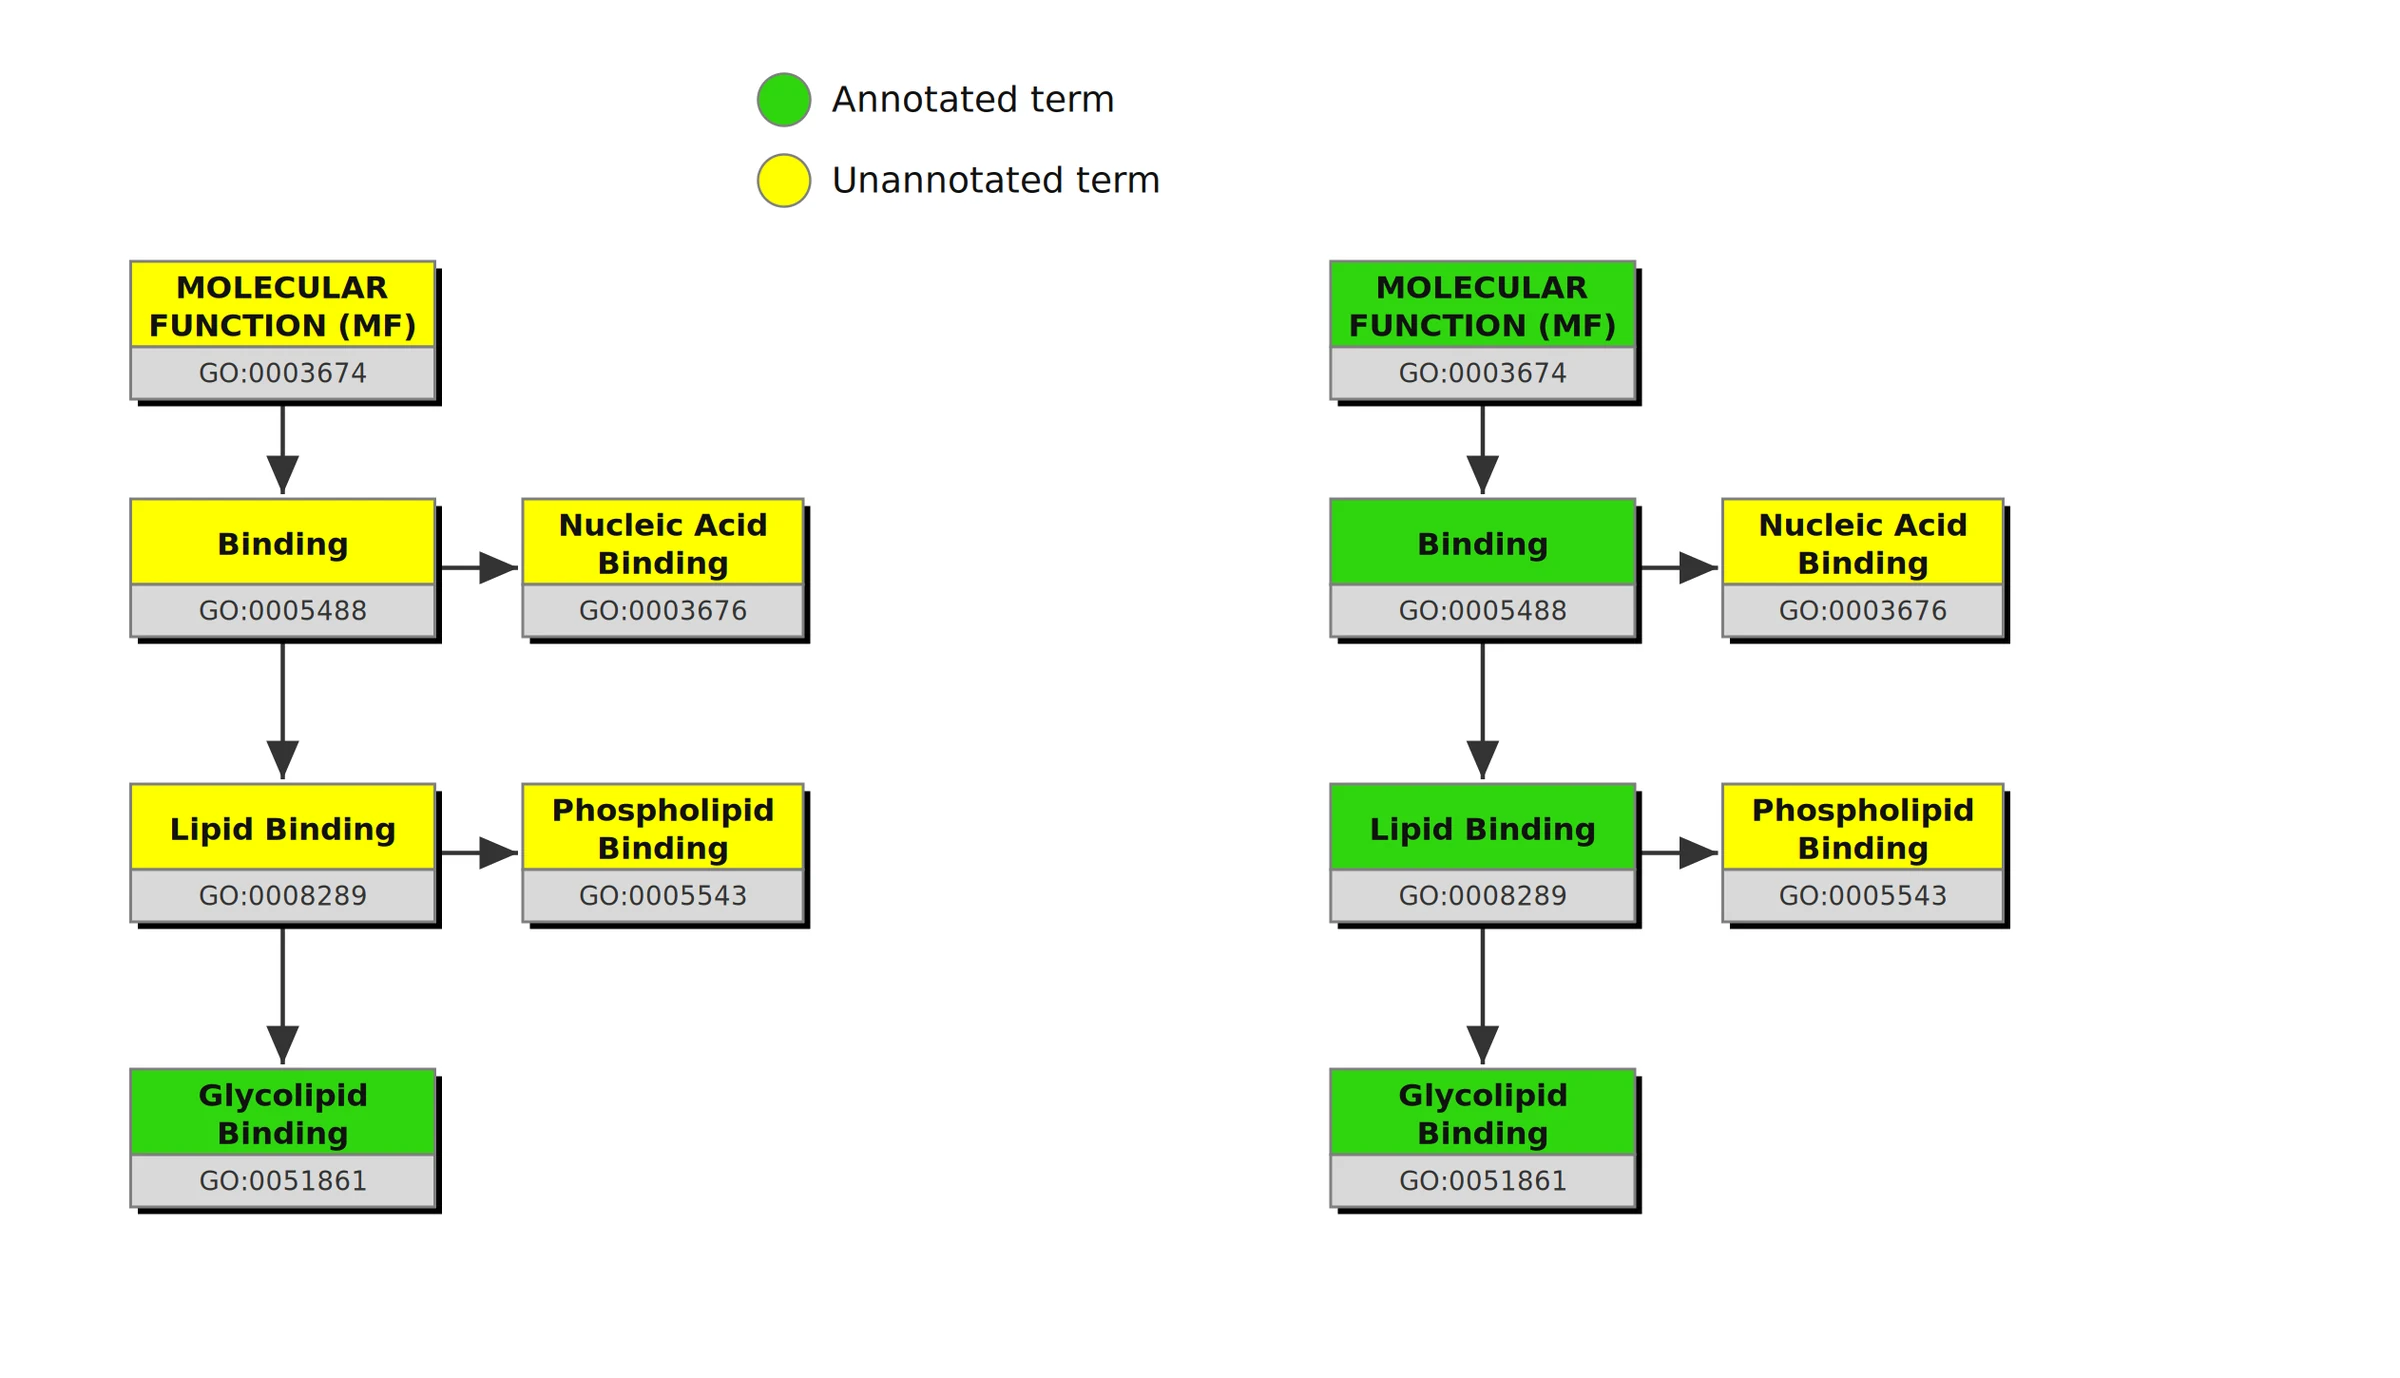
\includegraphics[width=\linewidth]{fig_2_1}
      \caption{Inconsistent (left) and consistent (right) annotation.}
    \end{figure}
  \end{columns}
\end{frame}

\begin{frame}{Function Also Depends on Context}
  \begin{columns}[c]
    \column{0.6\textwidth}
    \begin{itemize}\setlength{\itemsep}{0.4em}
      \item Proteins act in complexes and pathways
      \item PPI networks: nodes are proteins, edges are associations
      \item \textbf{Guilt by association:} connected proteins tend to share functions~\cite{vazquez_global_2003}
      \item STRING mixes evidence channels of uneven reliability~\cite{szklarczyk_string_2021}
      \item About one third of the proteins have no edge
    \end{itemize}
    \column{0.36\textwidth}
    \begin{figure}
      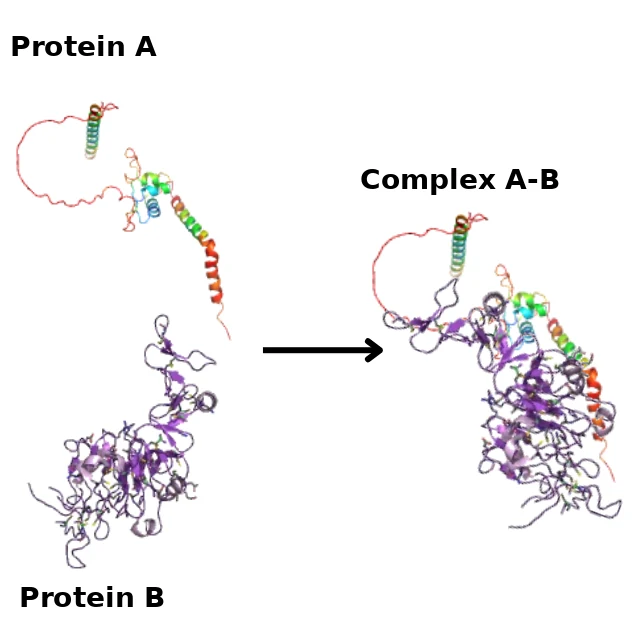
\includegraphics[width=0.8\linewidth]{fig_2_2}
      \caption{Two proteins forming a complex.}
    \end{figure}
  \end{columns}
\end{frame}

\begin{frame}{Problem Description}
  \begin{block}{Problem}
    Assign to each protein its Gene Ontology terms in BP, CC and MF, from its amino-acid sequence and its
    neighbourhood in the STRING network.
  \end{block}
  \vspace{0.6em}
  \begin{itemize}\setlength{\itemsep}{0.5em}
    \item About 500 terms per ontology, with the hierarchy respected
    \item One aggregated, cross-species network with heterogeneous evidence
    \item About one third of the proteins have no retained interaction, so a network-only model sees nothing for
      them
  \end{itemize}
\end{frame}

\begin{frame}{Objectives}
  \begin{block}{General objective}
    Develop, evaluate and combine approaches based on PPI networks for multi-label function annotation,
    integrating the network topology with amino-acid sequence embeddings.
  \end{block}
  \textbf{Specific objectives:}
  \begin{itemize}\small
    \item Compare representative network-based methods under one data and evaluation protocol
    \item Develop a fixed neighbourhood propagation, with no learned parameters
    \item Implement GNNs that aggregate the neighbourhood over protein language model features
    \item Compare vector, one-dimensional and image classification heads
    \item Combine fixed and GNN predictors with early and late fusion
    \item Benchmark against the state of the art; publish the results and the code
  \end{itemize}
\end{frame}

\begin{frame}{Research Questions}
  This work was guided by seven research questions:
  \vspace{0.3em}
  \begin{itemize}\setlength{\itemsep}{0.25em}
    \item \textbf{(RQ1)} Which representation of the STRING network works best?
    \item \textbf{(RQ2)} How much does propagating ProtT5 embeddings over STRING add?
    \item \textbf{(RQ3)} Fixed or learned aggregation, vector or image heads?
    \item \textbf{(RQ4)} Do early and late fusion improve on their components?
    \item \textbf{(RQ5)} How deep should the propagation go, and how much should a protein retain?
    \item \textbf{(RQ6)} How does the approach compare with the literature, on the same splits?
    \item \textbf{(RQ7)} Does it work on one global, aggregated-evidence network?
  \end{itemize}
\end{frame}

% =================================================================================== Background
\section{Theoretical Background}

\begin{frame}{Graphs, Adjacency and Message Passing}
  \begin{columns}[c]
    \column{0.44\textwidth}
    \begin{itemize}\setlength{\itemsep}{0.4em}
      \item $G=(V,E,w)$: proteins, associations, STRING confidence
      \item Adjacency matrix $A$; sparse storage in $O(|E|)$
      \item Message passing: aggregate the neighbours, then update the node
      \item $L$ layers reach $L$ hops; too many cause oversmoothing
    \end{itemize}
    \column{0.54\textwidth}
    \begin{figure}
      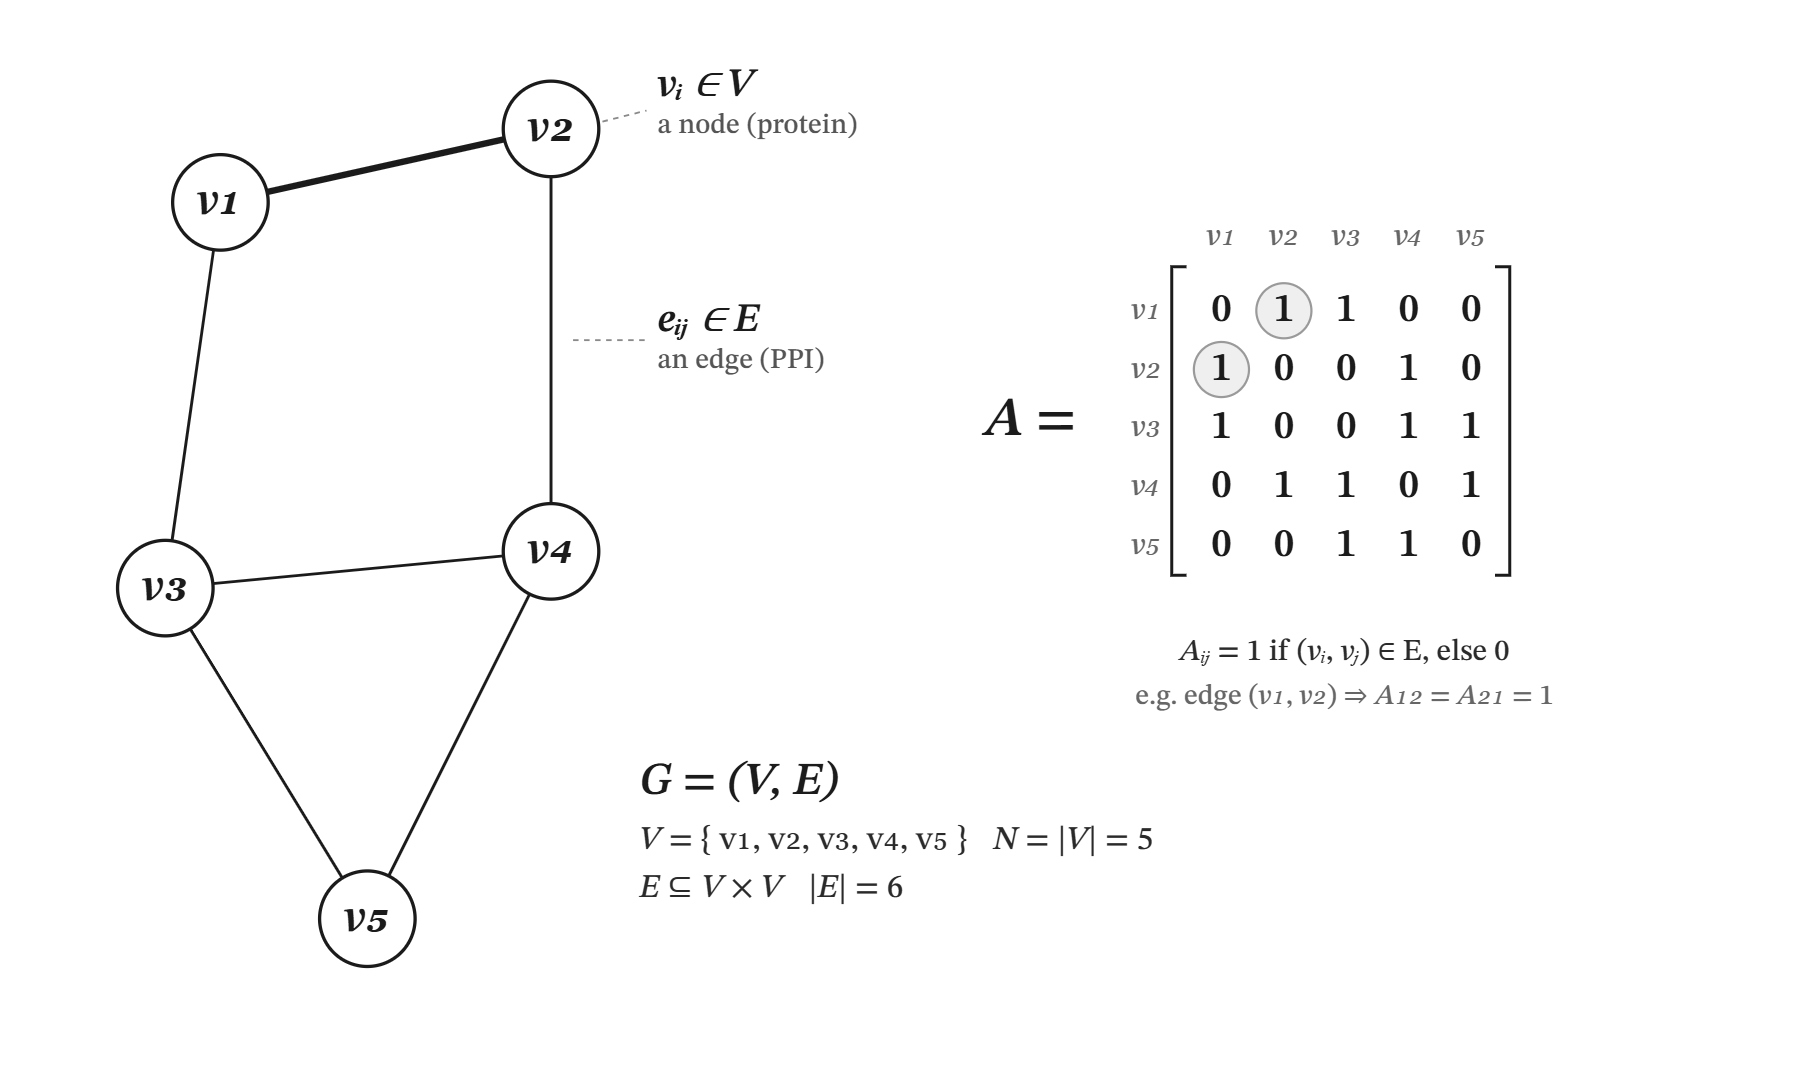
\includegraphics[width=\linewidth]{fig_2_3}
      \caption{Graph notation and adjacency matrix.}
    \end{figure}
  \end{columns}
\end{frame}

\begin{frame}{Graph Neural Networks: GCN and GAT}
  \begin{columns}[c]
    \column{0.47\textwidth}
    \begin{itemize}\setlength{\itemsep}{0.45em}
      \item \textbf{GCN}~\cite{kipf2017semi}: symmetric normalization of $W+I$, then a learned transform
      \item \textbf{GAT}~\cite{velickovic2018graph}: learned attention weights over the neighbours
      \item Used here: 2 layers, width 1024; GAT with 4 heads and the edge score as attribute
      \item Learned operators run on the full graph at every training step
    \end{itemize}
    \column{0.51\textwidth}
    \begin{eqbox}[\linewidth]
      $\displaystyle \mathbf{H}^{(\ell+1)}=\phi\Big(\tilde{D}^{-1/2}\,\tilde{W}\,\tilde{D}^{-1/2}\,\mathbf{H}^{(\ell)}\,\Theta^{(\ell)}\Big)$
      \\[0.9em]
      $\displaystyle a_{ij}=\frac{\exp(e_{ij})}{\sum_{k\in\mathcal{N}(i)\cup\{i\}}\exp(e_{ik})}$
    \end{eqbox}
    {\scriptsize $\tilde{W}=W+I$ and $\tilde{D}$ its degree matrix; $e_{ij}$ scores the pair $(i,j)$ from both
    endpoints and the edge.}
  \end{columns}
\end{frame}

\begin{frame}{Protein Language Models}
  \begin{itemize}\setlength{\itemsep}{0.5em}
    \item Self-supervised pretraining on very large collections of protein sequences
    \item Transformer encoder: every residue attends to every other
    \item \textbf{ProtT5-XL-U50}~\cite{elnaggar2021prottrans}: T5 encoder trained on BFD, then UniRef50, with 15\% of
      the residues masked
    \item Used here as a \alert{frozen} feature extractor
    \item A sequence embedding exists for every protein, with or without network edges
  \end{itemize}
\end{frame}

% =================================================================================== Related work
\section{Related Work}

\begin{frame}{From Neighbour Voting to Graph Transformers}
  \begin{center}
  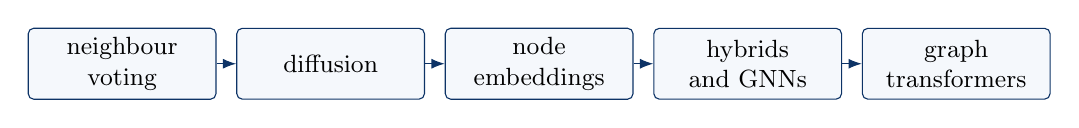
\begin{tikzpicture}[node distance=0.25cm, box/.style={draw=navy, rounded corners=2pt, align=center, font=\small,
      minimum height=0.9cm, text width=2.15cm, fill=blockbody}]
    \node[box] (a) {neighbour\\voting};
    \node[box, right=of a] (b) {diffusion};
    \node[box, right=of b] (c) {node\\embeddings};
    \node[box, right=of c] (d) {hybrids\\and GNNs};
    \node[box, right=of d] (e) {graph\\transformers};
    \foreach \x/\y in {a/b,b/c,c/d,d/e} \draw[-{Latex}, navy] (\x) -- (\y);
  \end{tikzpicture}
  \end{center}
  \vspace{0.3em}
  \begin{itemize}\setlength{\itemsep}{0.4em}
    \item Each step added parameters, tuning surface and cost
    \item Network-only methods cannot score a protein that is absent from the network
    \item Recent methods reach unseen proteins through homology search
  \end{itemize}
\end{frame}

\begin{frame}{Five Methods Reimplemented in This Work}
  \begin{table}\footnotesize
    \caption{Where each method keeps its learned parameters, and how it treats proteins outside the network.}
    \begin{tabular}{@{}lp{6.6cm}l@{}}\toprule
      Method & Learned parameters & Proteins outside the network \\ \midrule
      Mashup~\cite{cho2016compact} & none in the diffusion, all in the compression & not scored \\
      deepNF~\cite{deepnf} & none in the diffusion, all in the compression & not scored \\
      MELISSA~\cite{wu2024melissa} & labels injected into the network construction & not scored \\
      DeepGraphGO~\cite{you_deepgraphgo_2021} & between propagation steps & homology search \\
      SEGT-GO~\cite{wang2025segtgo} & in a transformer, after a non-parametric multi-hop aggregation & homology search \\
      \bottomrule
    \end{tabular}
  \end{table}
  \vspace{0.2em}
  All five were retrained on the same corpus, splits and transductive graph.
\end{frame}

\begin{frame}{Research Gap}
  \begin{alertblock}{Open question}
    \centering Is a learned graph component still needed once the propagated object is informative?
  \end{alertblock}
  \vspace{0.5em}
  \begin{itemize}\setlength{\itemsep}{0.45em}
    \item Proposal: propagate ProtT5 embeddings with a fixed, finite-step operator, then use an ordinary head
    \item A sequence representation exists for every protein, so the network adds instead of supplies
    \item No prior visual route starts from a propagated language-model embedding
  \end{itemize}
\end{frame}

% =================================================================================== Materials and methods
\section{Materials and Methods}

\begin{frame}{Dataset: a CAFA5-Derived Corpus}
  \begin{table}\small
    \caption{Proteins per split and retained terms per ontology.}
    \TabCorpus
  \end{table}
  \begin{itemize}\setlength{\itemsep}{0.3em}
    \item From the CAFA5 training data, as consolidated in previous work of the group~\cite{oliveira2025supermagov2}
    \item 80\,/\,10\,/\,10 split, disjoint at protein level, with no temporal or homology constraint
    \item Labels per protein (mean): 25.91 BP, 12.48 CC, 7.55 MF
    \item Label matrix density: 5.18\%, 2.51\%, 1.51\%
  \end{itemize}
\end{frame}

\begin{frame}{STRING v11.5: One Aggregated Network}
  \begin{columns}[c]
    \column{0.42\textwidth}
    \begin{itemize}\setlength{\itemsep}{0.4em}\small
      \item 2,422,234 records, 791,011 distinct pairs, 86,423 proteins
      \item Combined score in $[0.400, 0.999]$: confidence, not binding strength
      \item Each pair repeated 3.06 times on average (up to 170), always with the same score
      \item Heavy-tailed degree: median 5 to 7, maximum between 763 and 805
    \end{itemize}
    \column{0.56\textwidth}
    \begin{figure}
      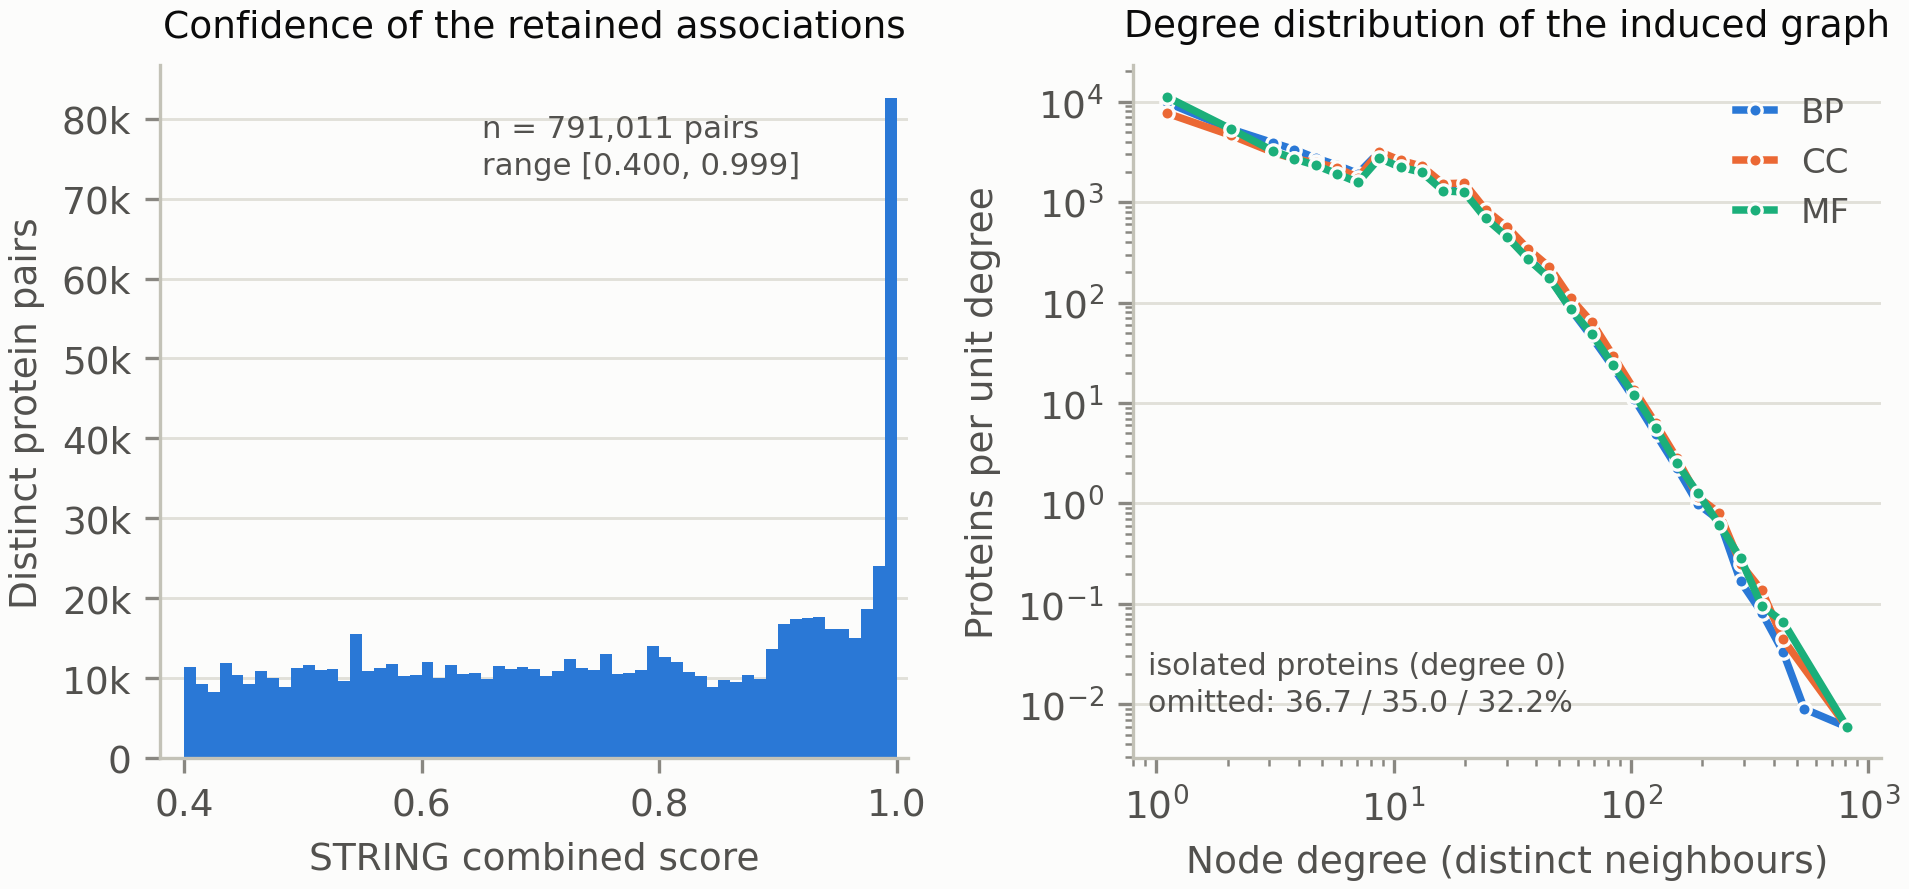
\includegraphics[width=\linewidth]{fig_4_1}
      \caption{Score of the retained pairs and degree distribution.}
    \end{figure}
  \end{columns}
\end{frame}

\begin{frame}{One Third of the Proteins Have No Edge}
  \begin{itemize}
    \item Isolated: 36.65\% BP, 34.95\% CC, 32.19\% MF; stable across training, validation and test
    \item Thresholds up to 0.40 are inert; at 0.90 more than half the proteins are isolated
  \end{itemize}
  \begin{columns}[c]
    \column{0.49\textwidth}
    \begin{figure}
      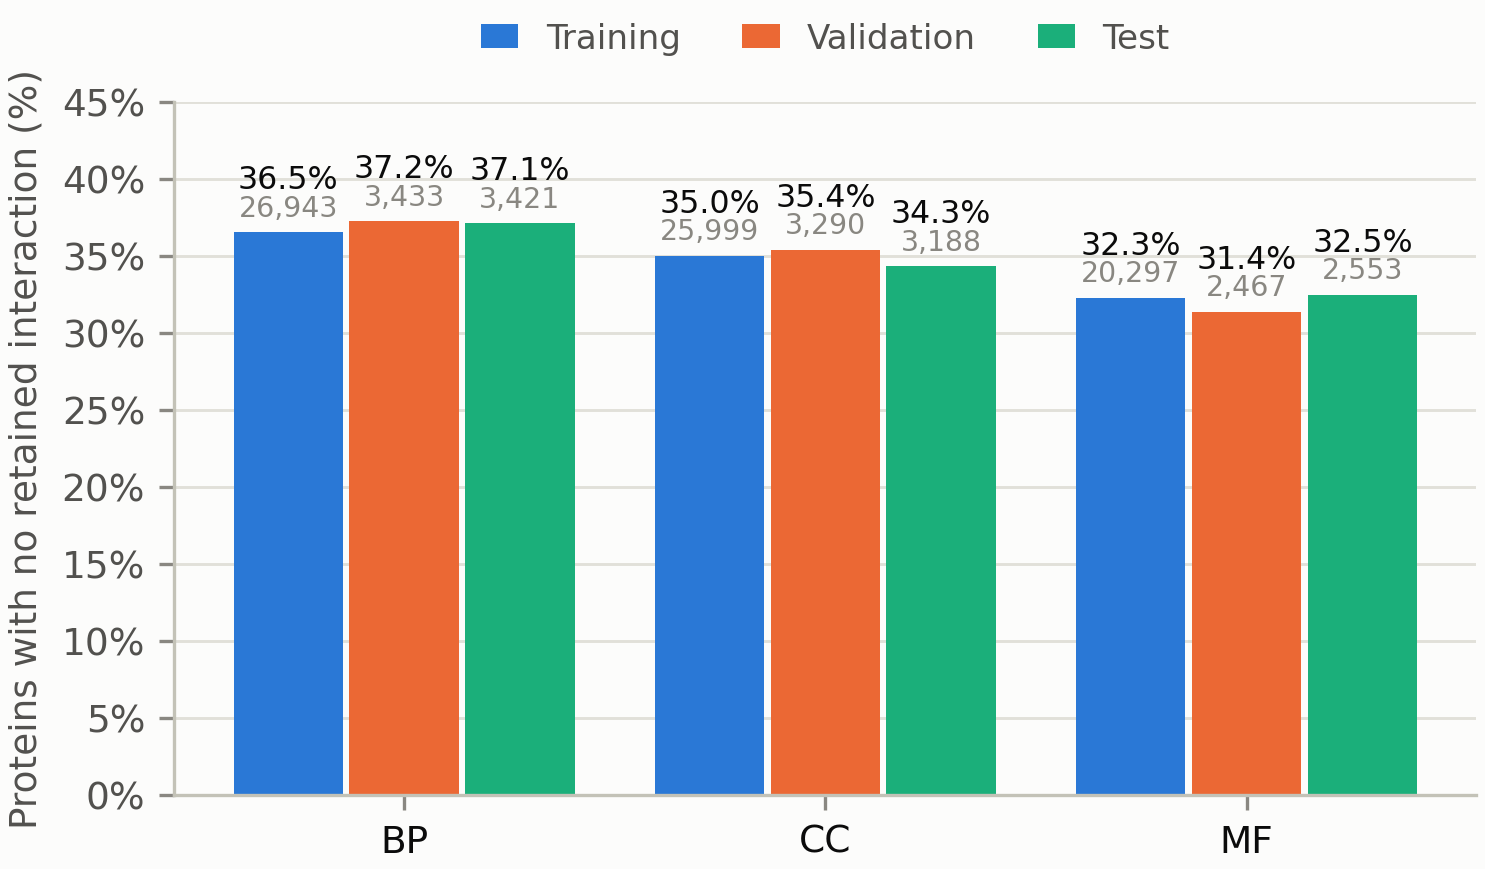
\includegraphics[width=0.9\linewidth]{fig_4_2}
      \caption{Isolated proteins per split.}
    \end{figure}
    \column{0.49\textwidth}
    \begin{figure}
      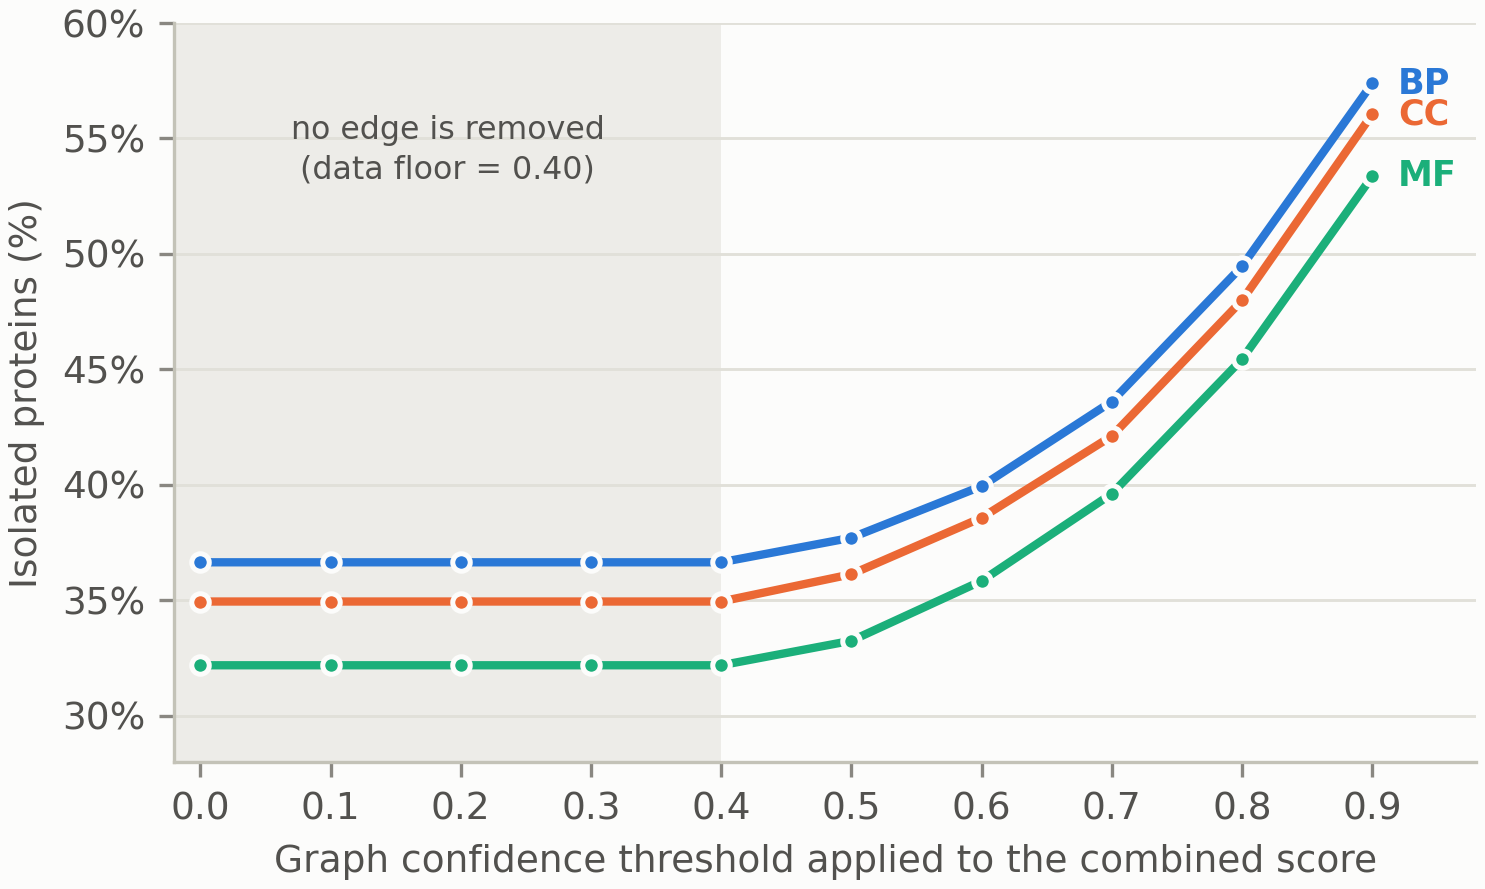
\includegraphics[width=0.9\linewidth]{fig_4_3}
      \caption{Isolated proteins against the score threshold.}
    \end{figure}
  \end{columns}
\end{frame}

\begin{frame}{Evaluation Metrics}
  \textbf{Primary criterion:} $\wF$, the $F$-measure weighted by information content (IC)
  \begin{eqbox}[0.86\textwidth]
    $\displaystyle \wF=\max_{\tau}\frac{2\,\mathrm{wpr}(\tau)\,\mathrm{wrc}(\tau)}{\mathrm{wpr}(\tau)+\mathrm{wrc}(\tau)},
    \qquad \mathrm{IC}(v)=-\log_2 P\big(v\mid \mathrm{pa}(v)\big)$
  \end{eqbox}
  \begin{itemize}\setlength{\itemsep}{0.35em}
    \item Also $F_{\max}$, $F^{*}_{\max}$ (root excluded), $\Smin$ (bits, lower is better), AuPRC and IAuPRC
    \item Predictions made consistent with the hierarchy before scoring
    \item 101 thresholds; full evaluation mode: an unpredicted protein counts as zero recall
  \end{itemize}
\end{frame}

\begin{frame}{Experimental Protocol}
  \begin{figure}
    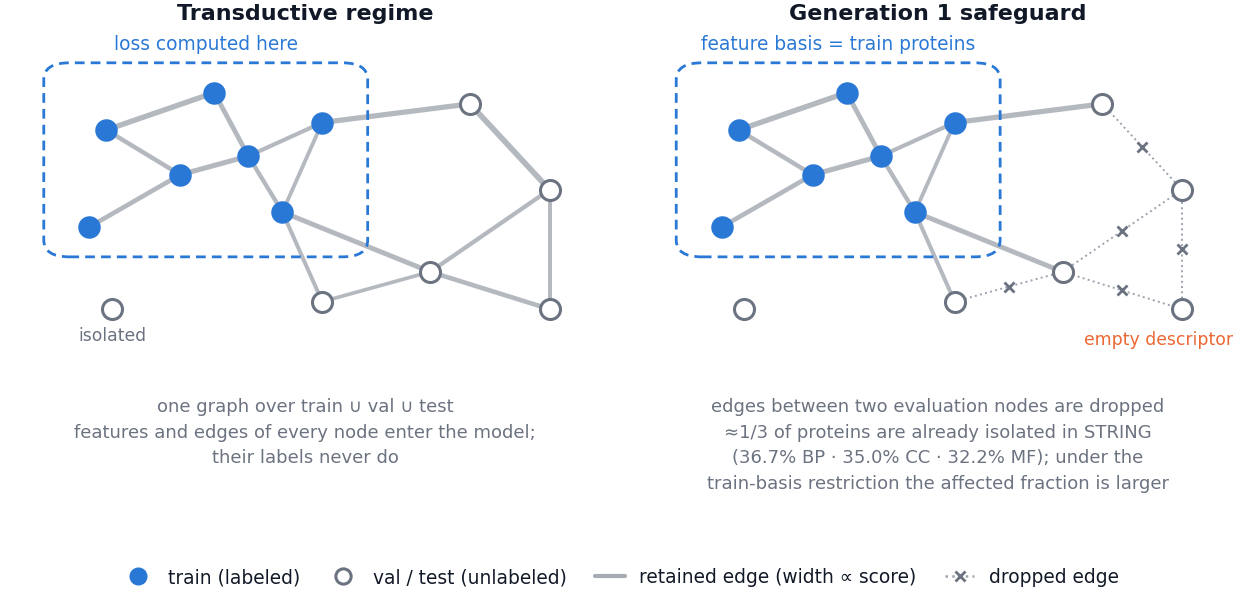
\includegraphics[height=0.46\textheight]{fig_5_2}
    \caption{Transductive regime: one graph over all proteins, labels read only for training proteins.}
  \end{figure}
  \begin{itemize}\setlength{\itemsep}{0.3em}
    \item Every design decision taken on validation; the test set read once, at the end
    \item Single seed: differences below 0.5\,pp are read as ties
  \end{itemize}
\end{frame}

\begin{frame}{Methodology: Two Generations, Three Decisions}
  \begin{columns}[c]
    \column{0.34\textwidth}
    \begin{itemize}\setlength{\itemsep}{0.45em}
      \item Every model: representation, propagation, prediction head
      \item Generation 1: the network alone
      \item About one third isolated: null descriptor
      \item Generation 2 (NEXUS-GO): ProtT5 plus the network
    \end{itemize}
    \column{0.64\textwidth}
    \begin{figure}
      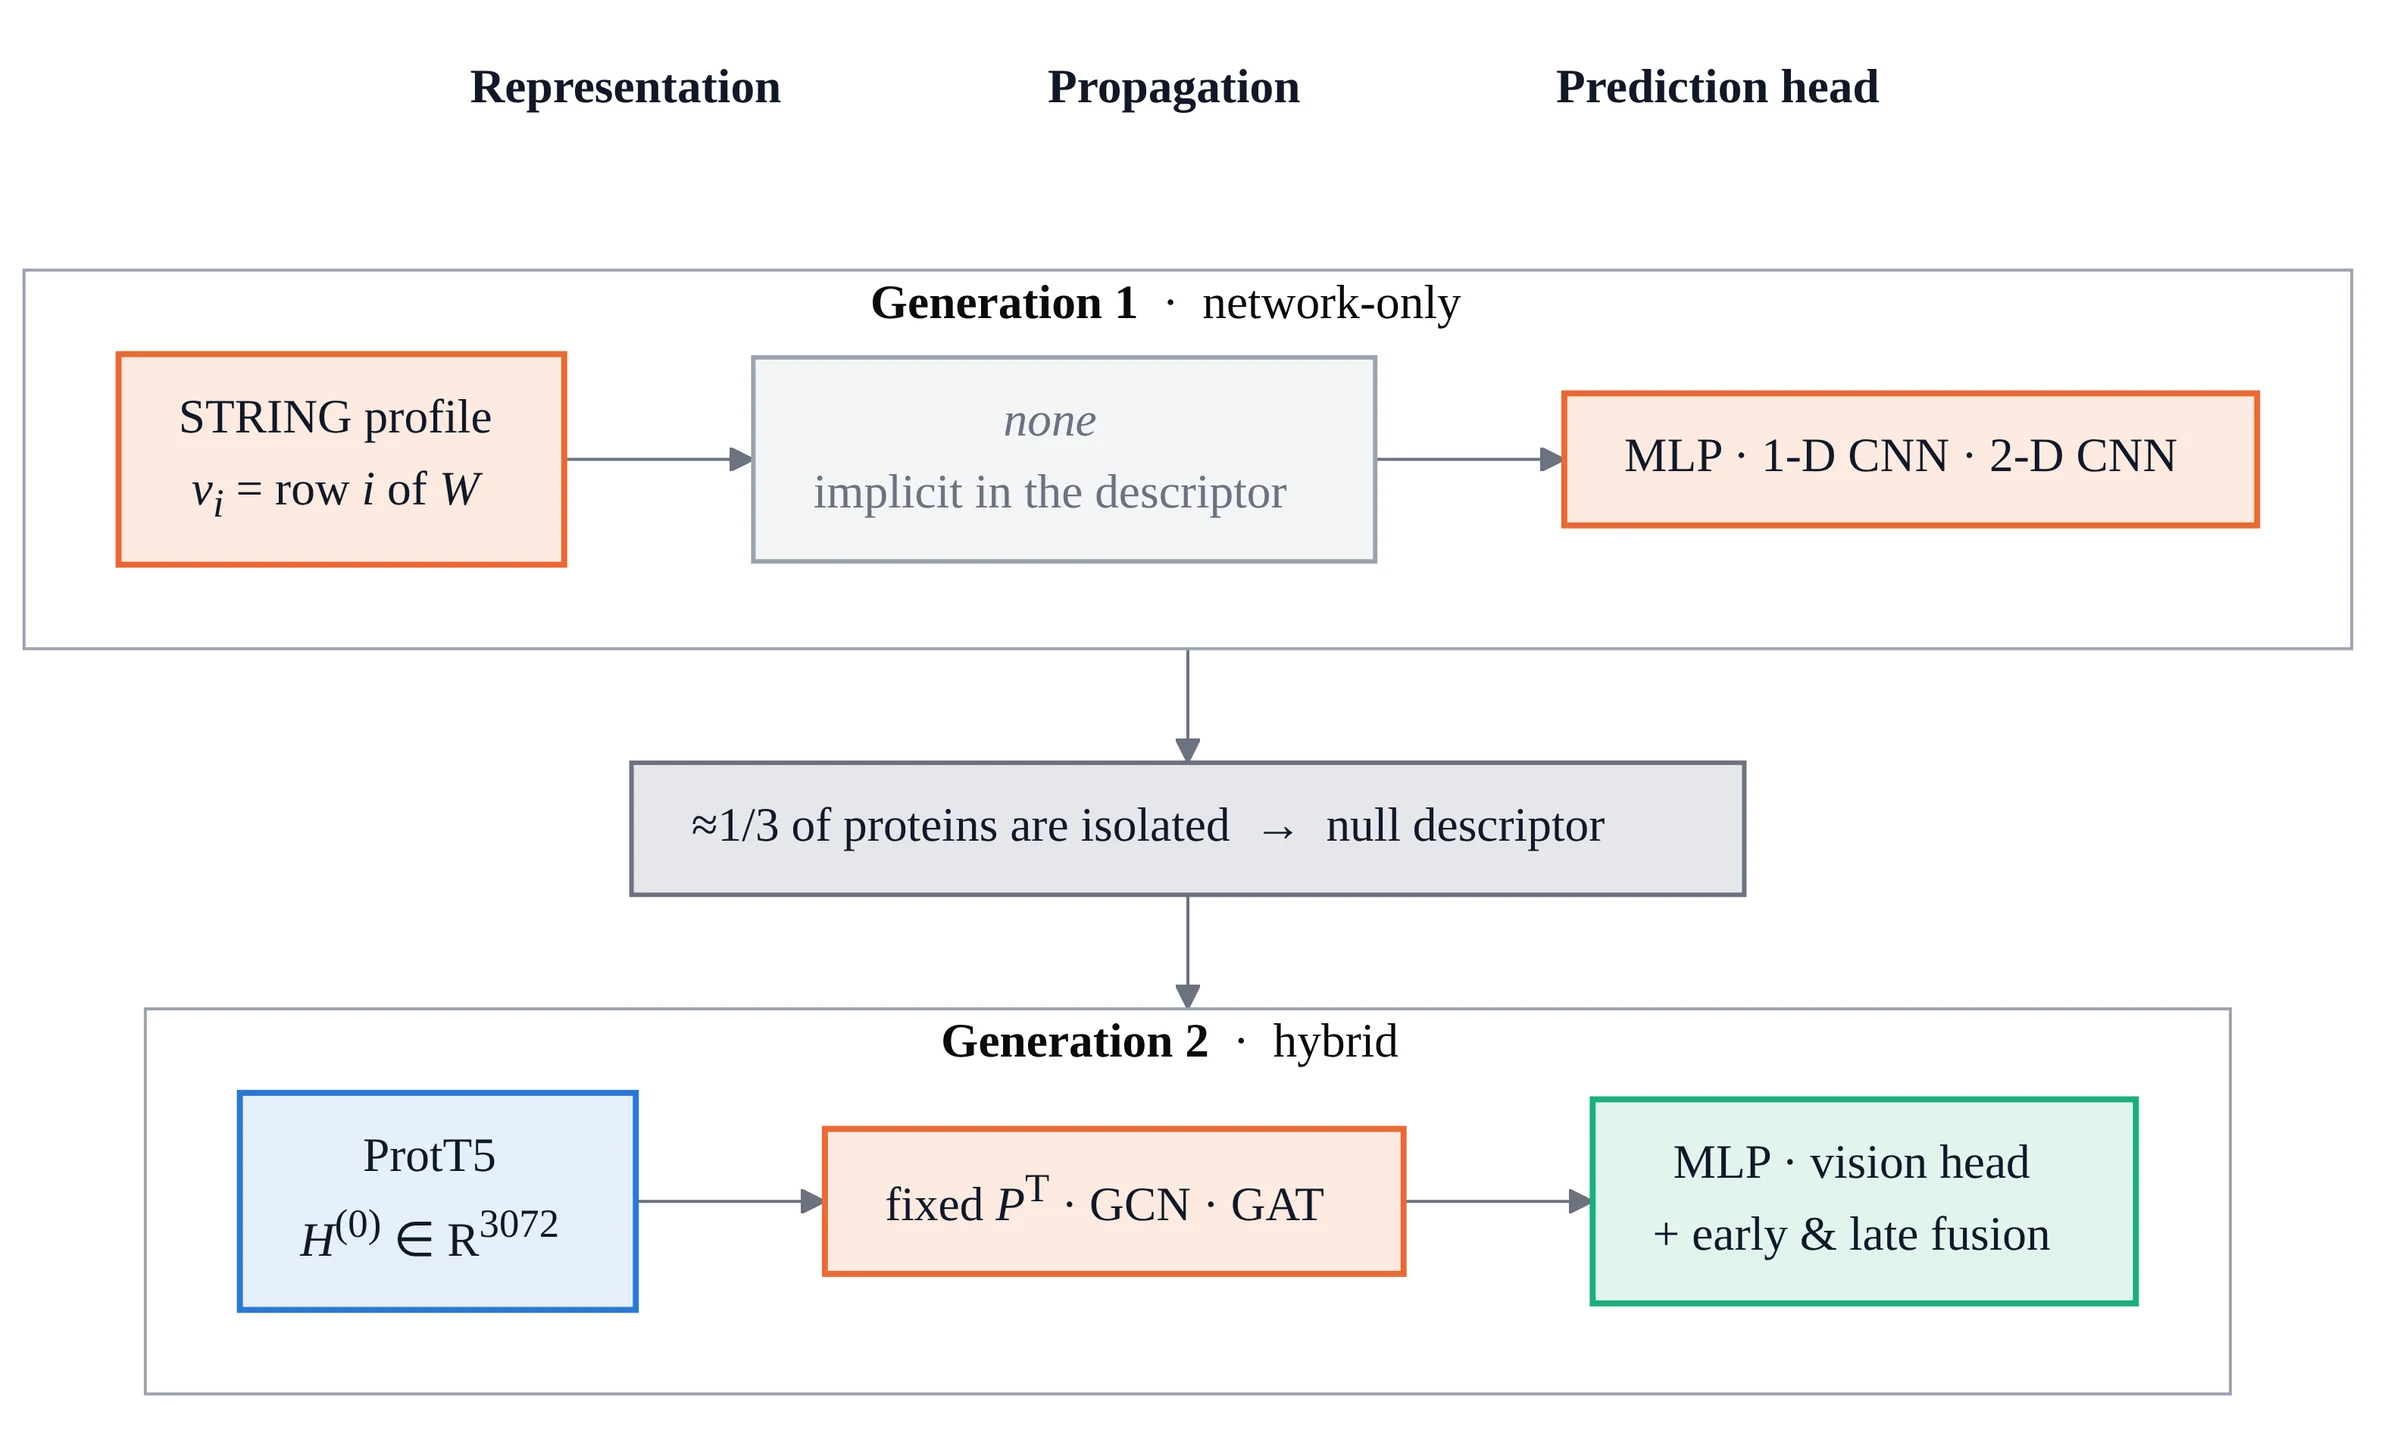
\includegraphics[width=\linewidth]{fig_5_1}
      \caption{The two generations along the three decisions.}
    \end{figure}
  \end{columns}
\end{frame}

\begin{frame}{Generation 1: the Network Alone}
  \begin{columns}[c]
    \column{0.18\textwidth}
    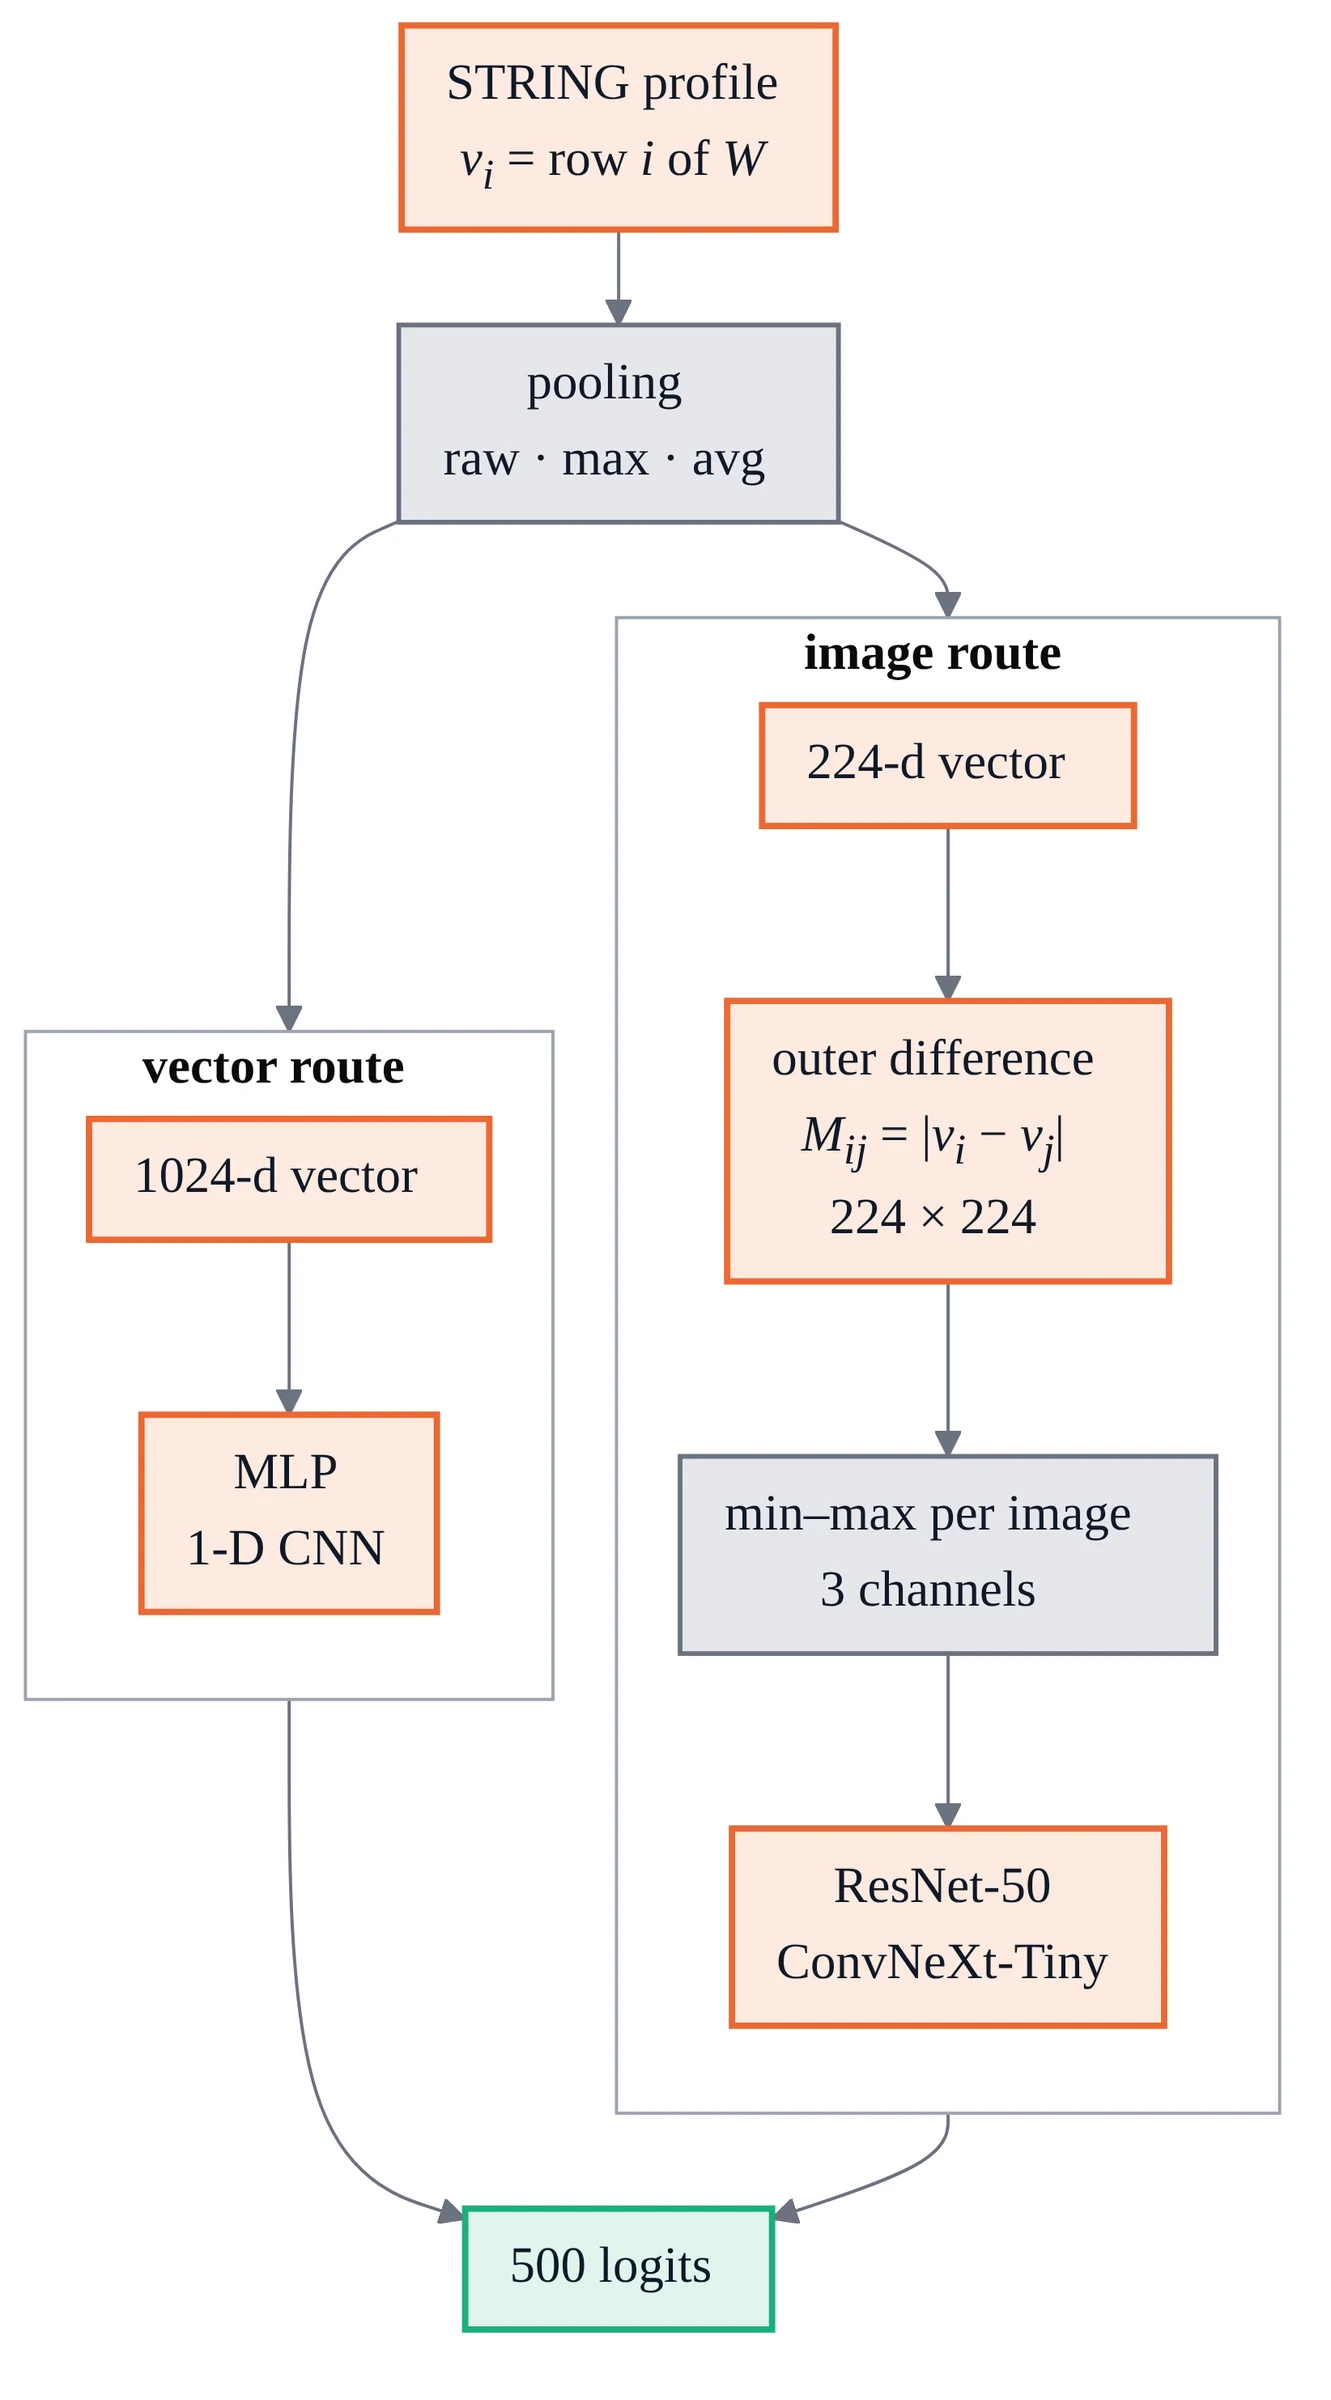
\includegraphics[width=\linewidth, height=0.72\textheight, keepaspectratio]{fig_5_3}
    \column{0.8\textwidth}
    \begin{itemize}\setlength{\itemsep}{0.2em}\small
      \item Input: the protein's row of the weighted adjacency, against the training proteins
      \item Pooling: raw, max or avg; vector route: MLP or 1-D CNN
      \item Image route: outer-difference matrix $|v_i-v_j|$, $224\times224$, ResNet-50 or ConvNeXt-Tiny
      \item Floor: a naive term-frequency baseline
    \end{itemize}
    \begin{figure}
      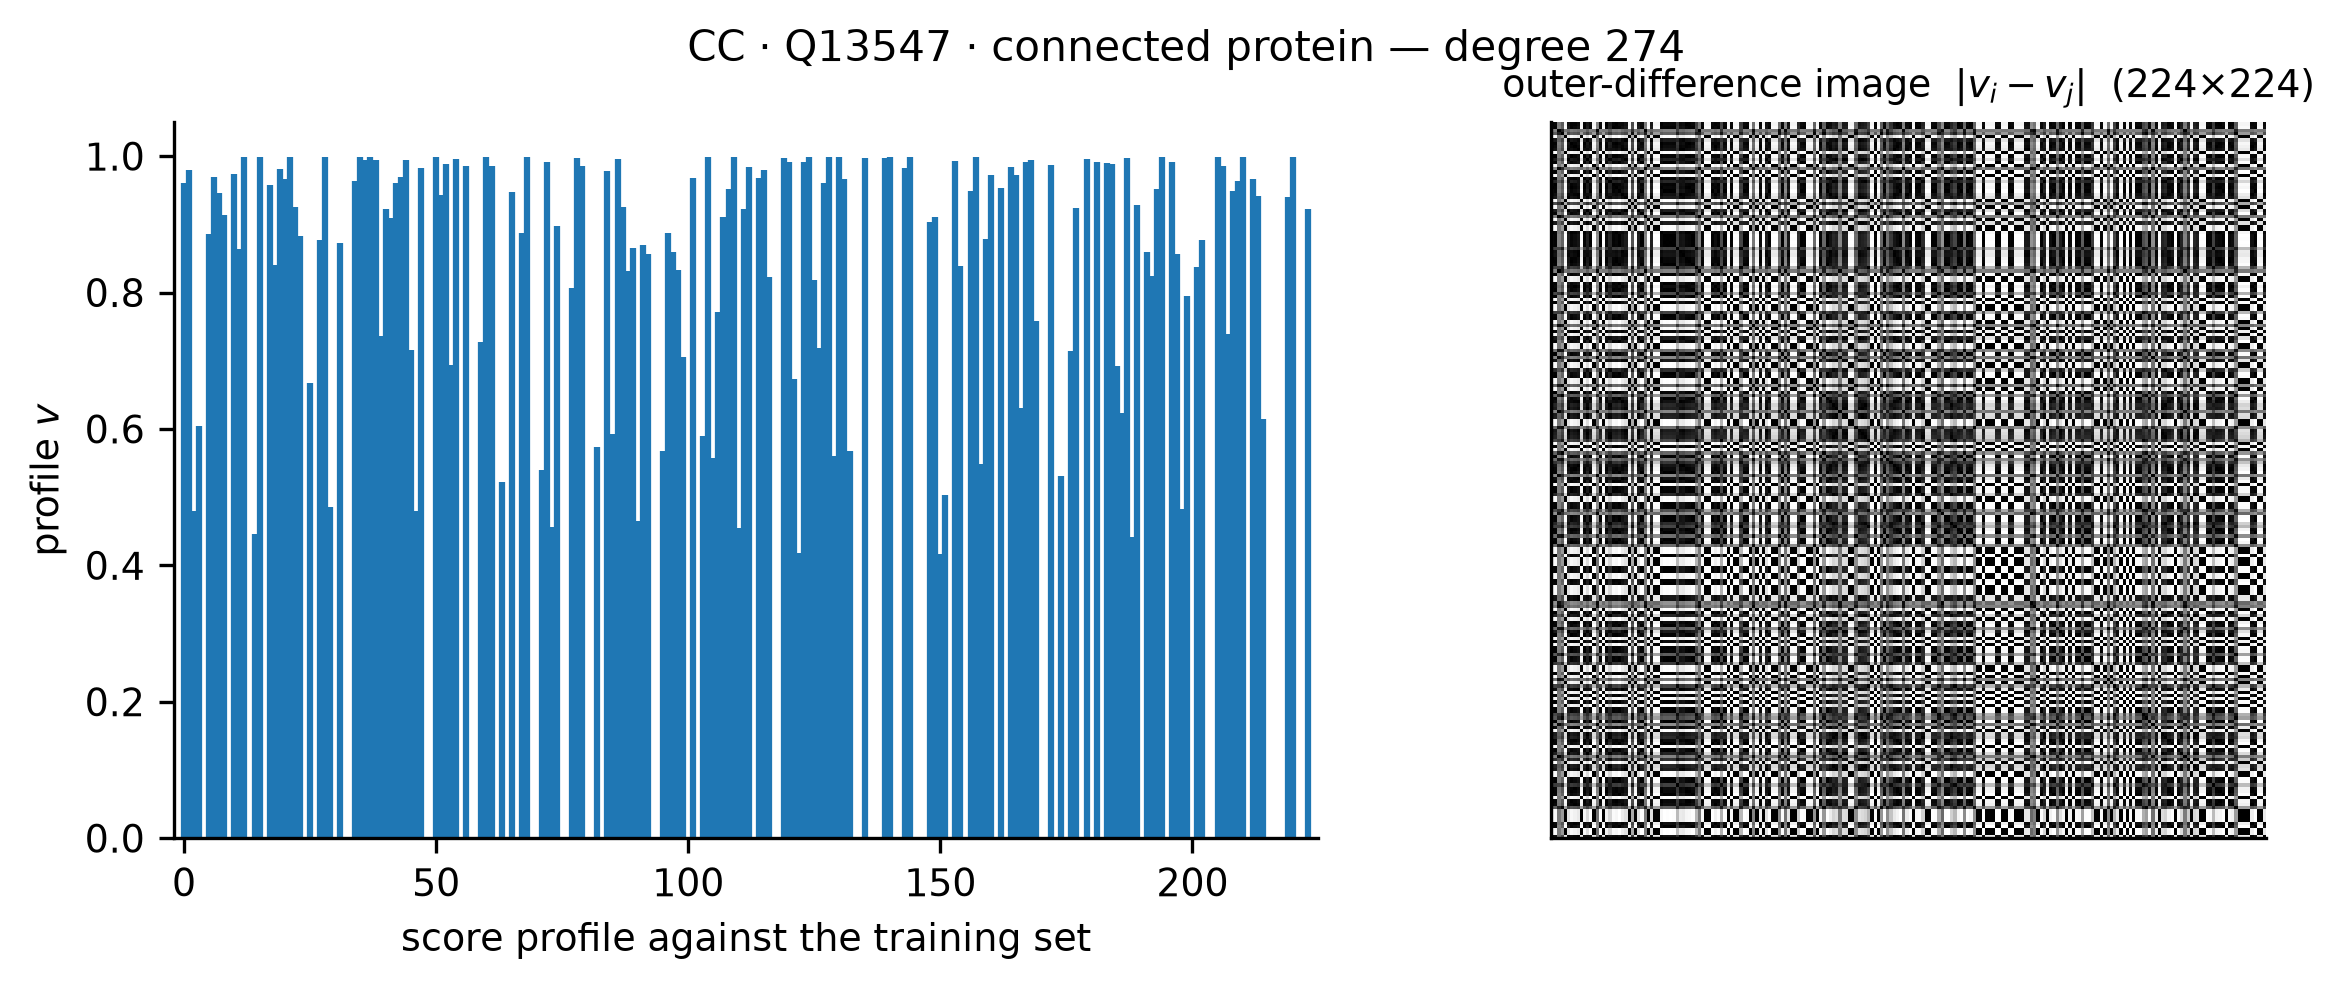
\includegraphics[height=0.32\textheight]{fig_5_4}
      \caption{A connected protein: its profile and its outer-difference image.}
    \end{figure}
  \end{columns}
\end{frame}

\begin{frame}{An Isolated Protein Has No Input}
  \begin{figure}
    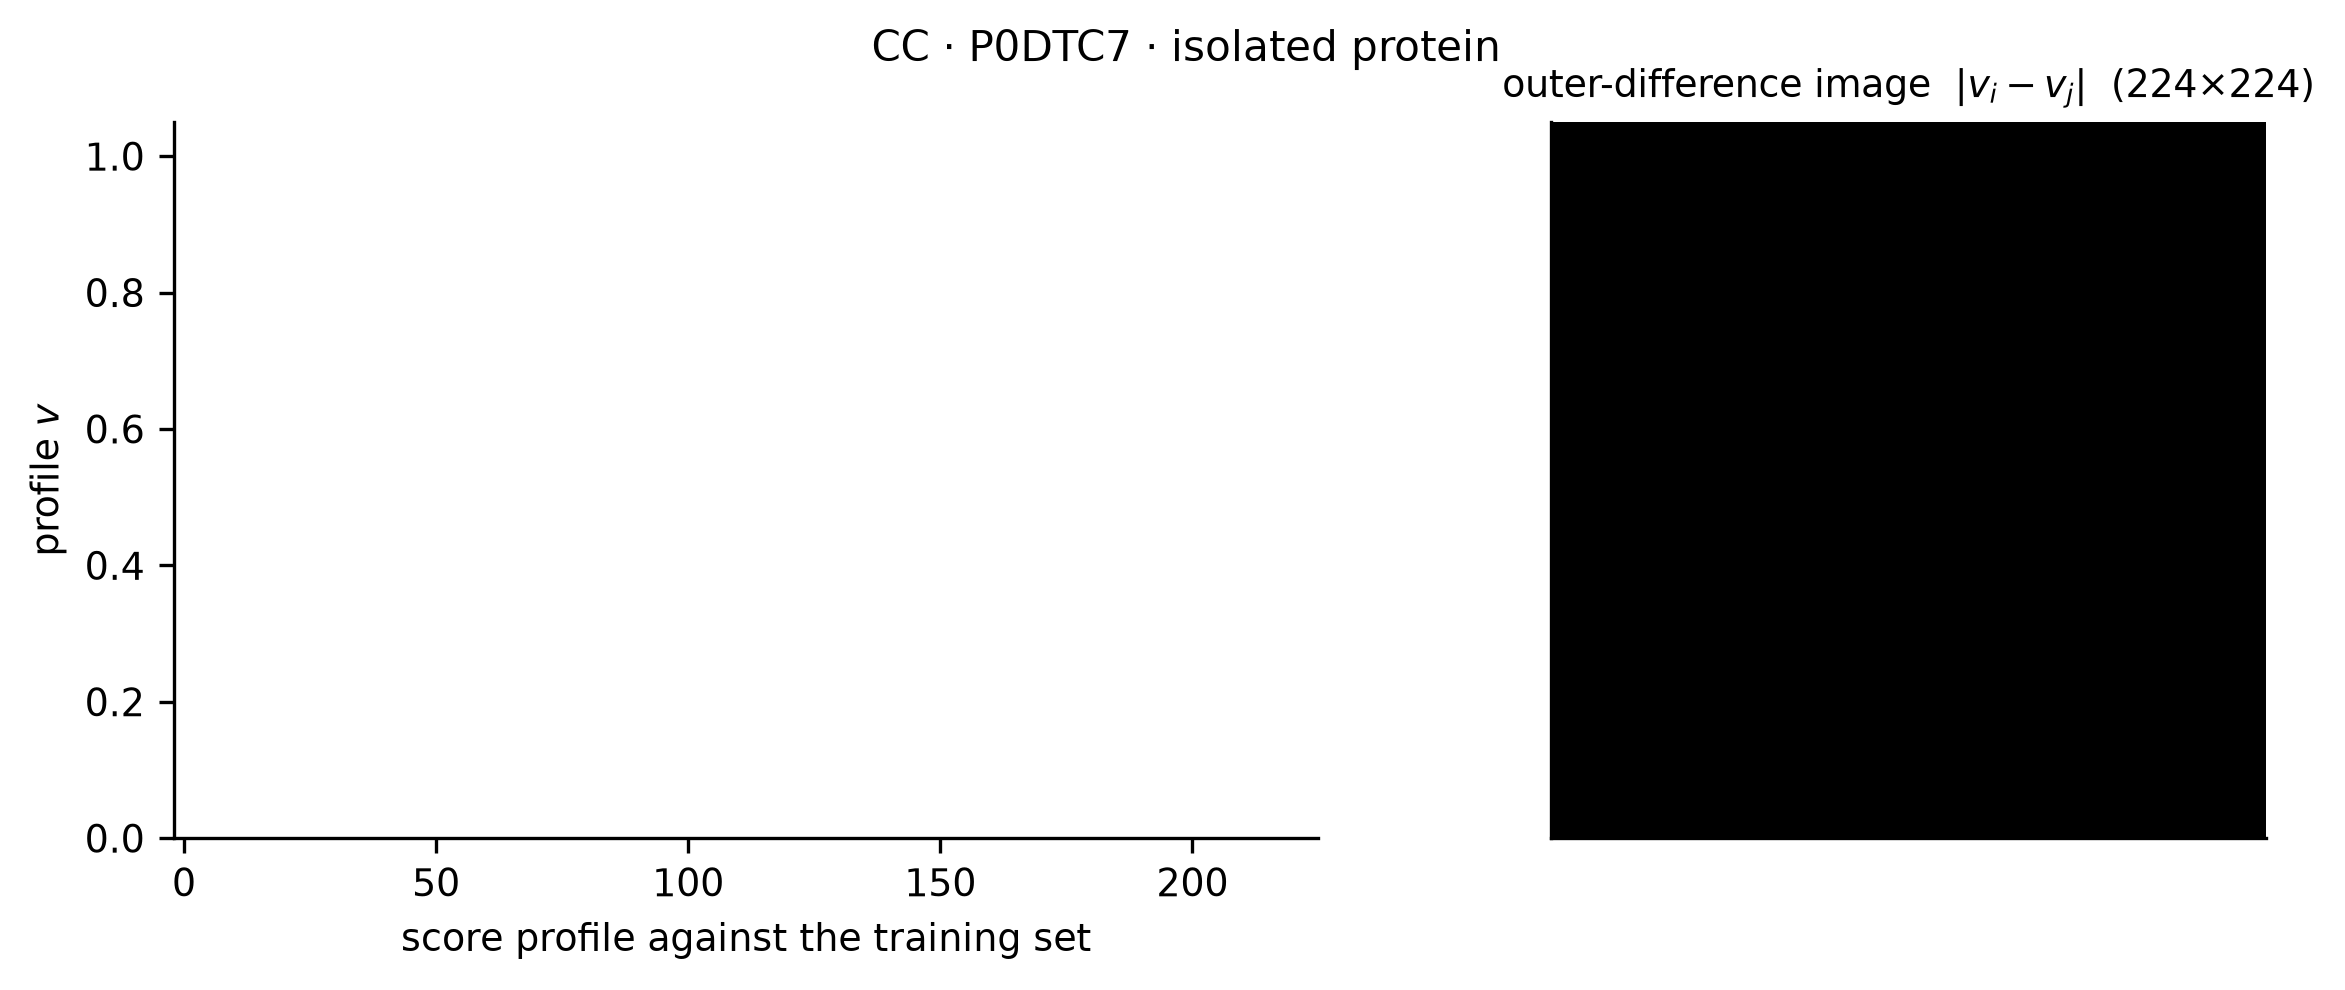
\includegraphics[height=0.42\textheight]{fig_5_5}
    \caption{An isolated protein: a null profile and a uniform image.}
  \end{figure}
  \begin{itemize}\setlength{\itemsep}{0.3em}
    \item Null profile, null matrix, uniform image: the head can only return the class prior
    \item No architecture can recover what is absent
    \item \alert{Requirement: a representation that exists for every protein}
  \end{itemize}
\end{frame}

\begin{frame}{NEXUS-GO: Four Routes}
  \begin{center}
  \begin{tikzpicture}[font=\small, >={Latex},
      b/.style={draw, rounded corners=2pt, align=center, minimum height=0.8cm, inner sep=4pt},
      r/.style={b, draw=navy, fill=blockbody, text width=2.9cm}]
    \node[b, draw=seq, text=seq] (seq) at (0,1.2) {Sequence};
    \node[b, draw=seq, text=seq, right=0.6cm of seq] (pt5) {ProtT5\\$H^{(0)}\in\mathbb{R}^{3072}$};
    \node[b, draw=net, text=net] (str) at (0,-1.2) {STRING};
    \node[b, draw=net, text=net, right=0.6cm of str] (w) {graph $W$\\$P=W D_c^{-1}$};
    \draw[->, seq] (seq) -- (pt5); \draw[->, net] (str) -- (w);
    \node[r, right=1.4cm of pt5, yshift=-0.2cm] (fix) {\NX{Fixed}\\fixed propagation};
    \node[r, right=1.4cm of w, yshift=0.2cm] (gnn) {\NX{GNN}\\learned (GCN, GAT)};
    \draw[->] (pt5) -- (fix); \draw[->] (w) -- (fix.west);
    \draw[->] (pt5) -- (gnn.west); \draw[->] (w) -- (gnn);
    \node[r, draw=fus, fill=fus!8, right=1.2cm of fix, yshift=-0.85cm] (early) {\NX{Early}\\join representations};
    \node[r, draw=fus, fill=fus!8, below=0.25cm of early] (late) {\NX{Late}\\combine probabilities};
    \draw[->, fus] (fix.east) -- (early.west); \draw[->, fus] (gnn.east) -- (early.west);
    \draw[->, fus] (fix.east) -- (late.west); \draw[->, fus] (gnn.east) -- (late.west);
    \only<2>{\node[hl, fit=(seq)(pt5)(str)(w)] {};}
    \only<3>{\node[hl, fit=(fix)] {};}
    \only<4>{\node[hl, fit=(gnn)] {};}
    \only<5>{\node[hl, fit=(early)(late)] {};}
  \end{tikzpicture}
  \end{center}
  \vspace{0.4em}
  \begin{overprint}
    \onslide<1>\centering Two inputs and four routes; Generation 1 stays as a topology-only control.
    \onslide<2>\centering ProtT5 exists for every protein; STRING gives the weighted graph $W$ and the operator $P$.
    \onslide<3>\centering \NX{Fixed}: propagation with no parameters, computed once and cached.
    \onslide<4>\centering \NX{GNN}: GCN or GAT, recomputed at every training step.
    \onslide<5>\centering \NX{Early} joins the two representations; \NX{Late} combines their probabilities.
  \end{overprint}
\end{frame}

\begin{frame}{ProtT5-XL-U50: Three Layers, Frozen}
  \begin{figure}
    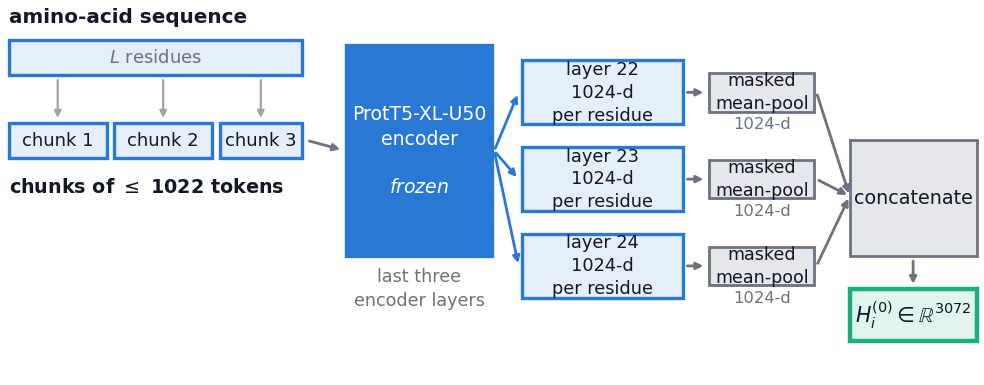
\includegraphics[width=0.66\linewidth]{fig_5_7}
    \caption{Extraction of the ProtT5 representation.}
  \end{figure}
  \begin{itemize}\setlength{\itemsep}{0.3em}
    \item Chunks of at most 1,022 residues; masked mean-pool, then mean over the chunks
    \item Layers 24, 23 and 22, concatenated: $3\times1024=3072$ dimensions
    \item Exists for every protein, isolated or not
  \end{itemize}
\end{frame}

\begin{frame}{Fixed Propagation: No Parameters}
  \begin{eqbox}[0.84\textwidth]
    $\displaystyle H^{(h)} = \alpha\,H^{(h-1)} + (1-\alpha)\,P^{\top}H^{(h-1)},\qquad h=1,\dots,T$
    \\[0.7em]
    $\displaystyle H^{(T)} = \sum_{k=0}^{T}\binom{T}{k}\,\alpha^{T-k}(1-\alpha)^{k}\,\big(P^{\top}\big)^{k}H^{(0)}$
  \end{eqbox}
  \begin{itemize}\setlength{\itemsep}{0.3em}\small
    \item $P = W D_c^{-1}$ is column-stochastic: weights are relative to each protein's neighbours
    \item Duplicate STRING records merged with \textbf{max}, which keeps the score (sum would multiply it)
    \item Computed once, cached, reused every epoch; $T=0$ or $\alpha=1$ switches the graph off
    \item Unlike personalized PageRank, the initial state is never reintroduced
  \end{itemize}
\end{frame}

\begin{frame}{Propagation on Four Real Proteins}
  \begin{columns}[c]
    \column{0.56\textwidth}
    \begin{figure}
      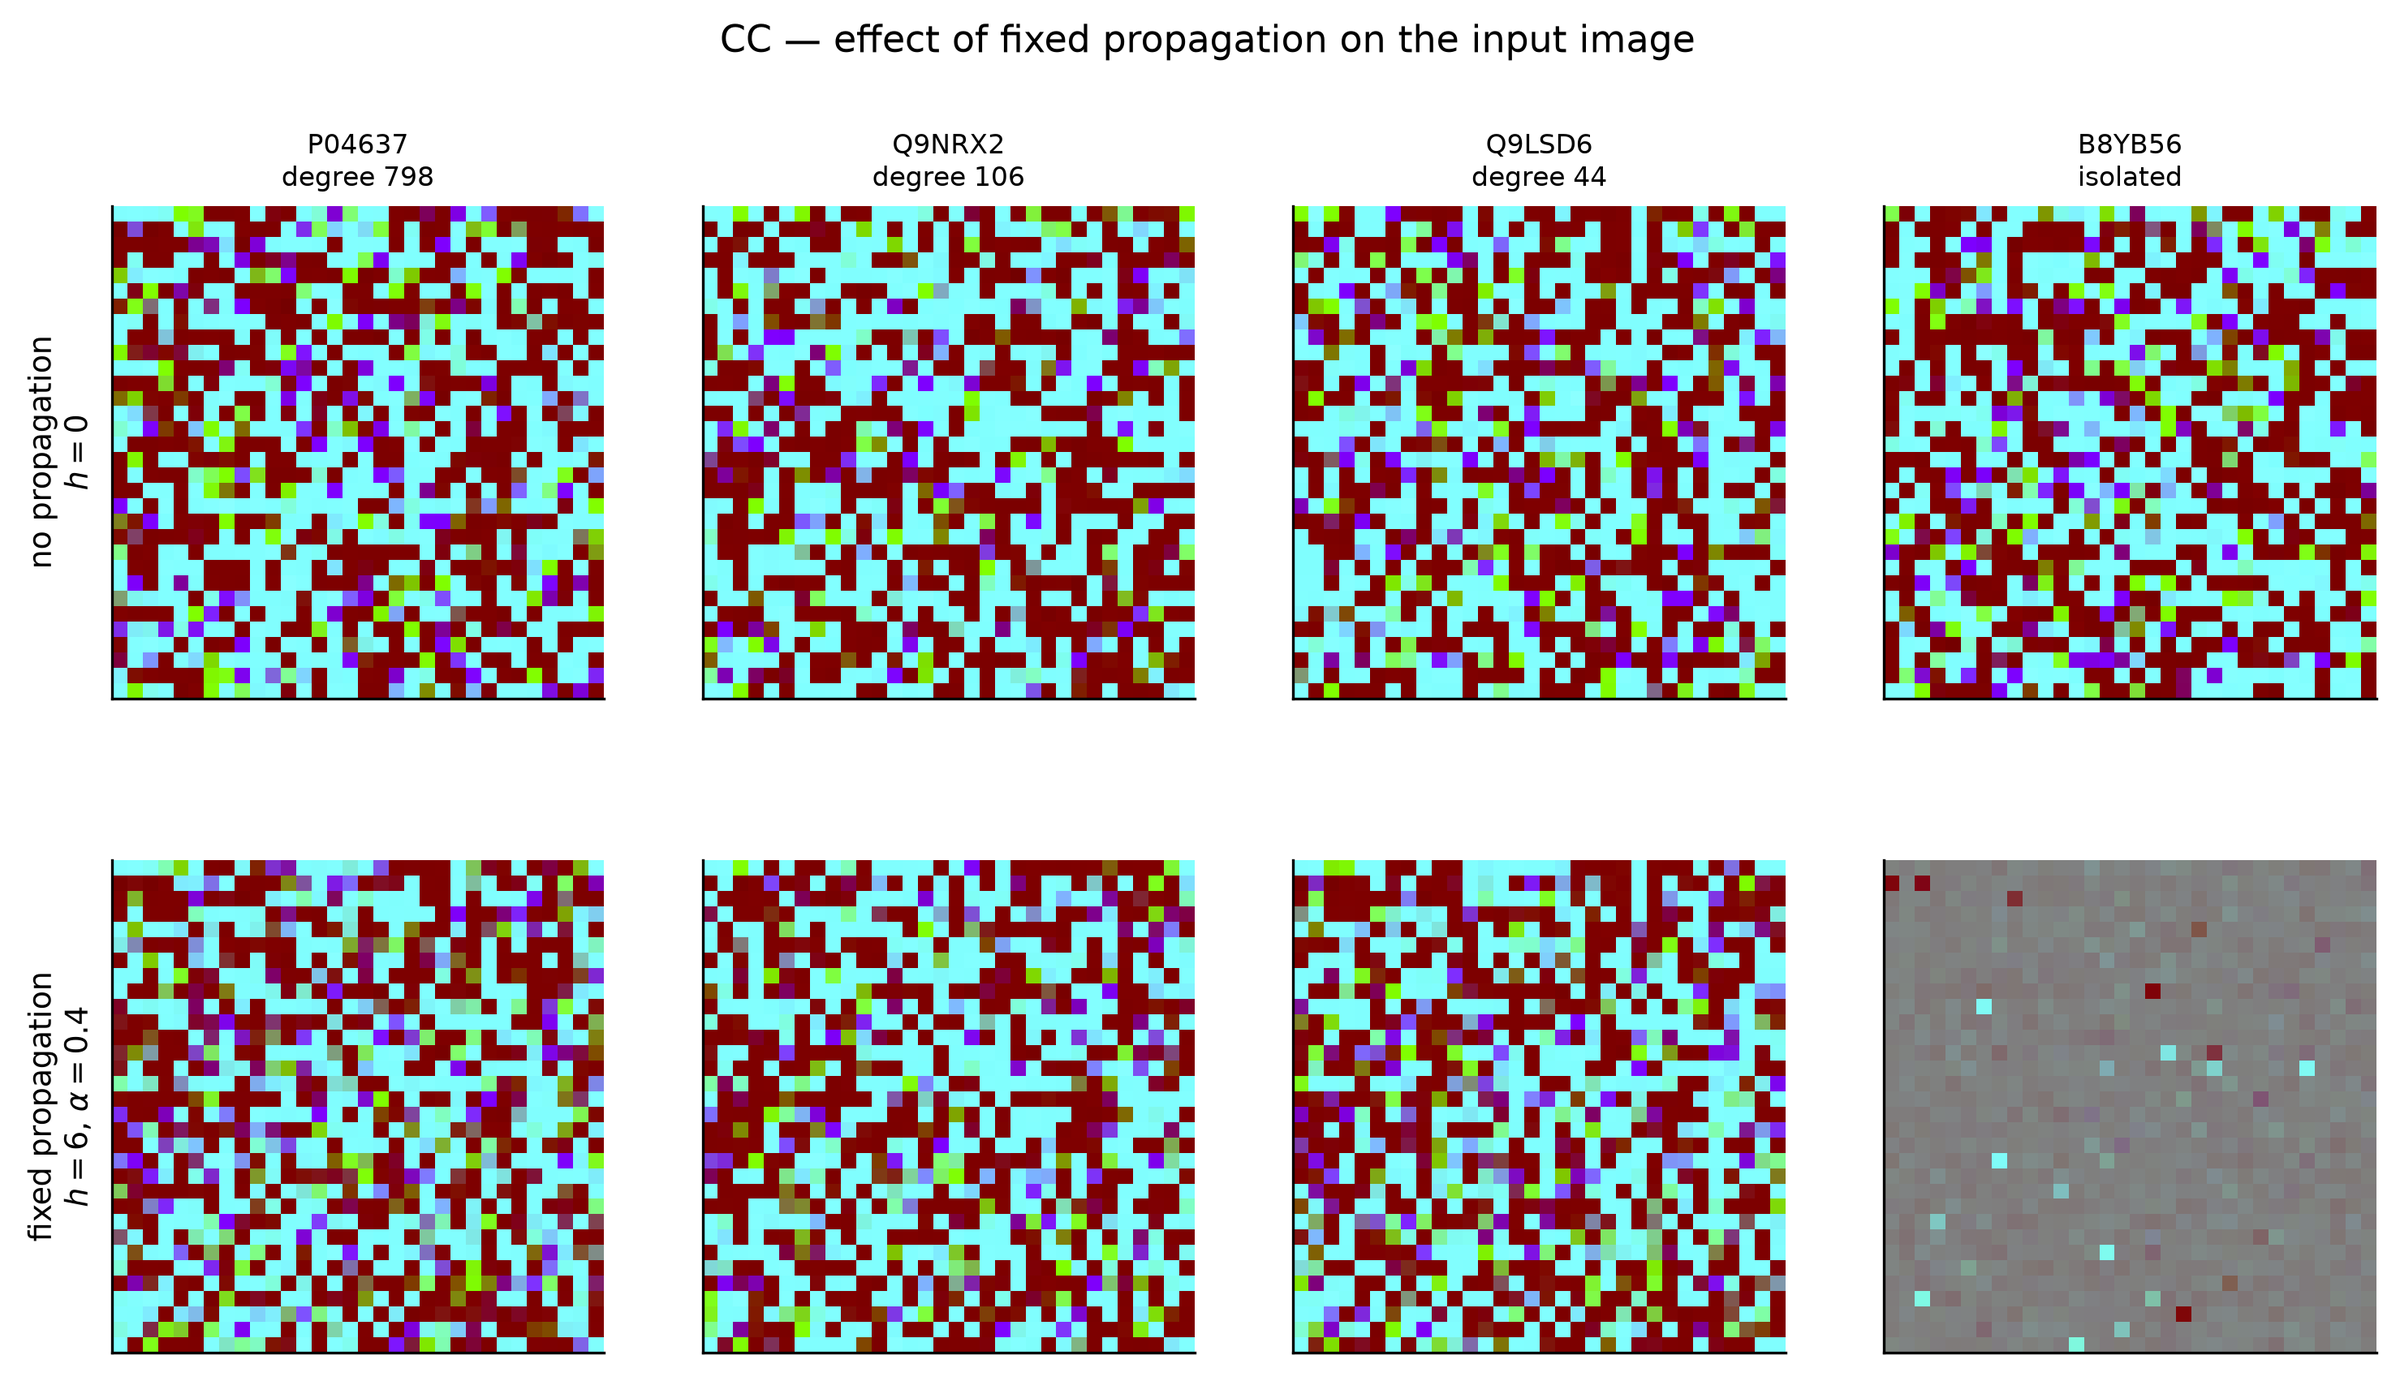
\includegraphics[width=\linewidth]{fig_5_8}
      \caption{CC images of four proteins: $T=0$ (top) and $T=6$, $\alpha=0.4$ (bottom).}
    \end{figure}
    \column{0.42\textwidth}
    \begin{itemize}\setlength{\itemsep}{0.45em}
      \item Connected proteins keep their structure and absorb their neighbourhood
      \item An isolated protein becomes $\alpha^{T}H^{(0)}$: same direction, smaller scale
      \item So its gains cannot come from neighbourhood information
    \end{itemize}
  \end{columns}
\end{frame}

\begin{frame}{Prediction Heads: Vector and Vision}
  \begin{itemize}\setlength{\itemsep}{0.25em}
    \item \textbf{Vector:} MLP $[1024, 512]$, batch normalization, dropout 0.4
    \item \textbf{Vision:} $\sigma(\mathrm{clip}(z))$ split into three $32\times32$ channels, one per ProtT5 layer
    \item Backbones: ResNet-50~\cite{he2016deep} and ConvNeXt-Tiny~\cite{liu2022convnet} (ImageNet), fully fine-tuned
    \item \alert{Caution:} pixel adjacency has no meaning in these images
  \end{itemize}
  \begin{figure}
    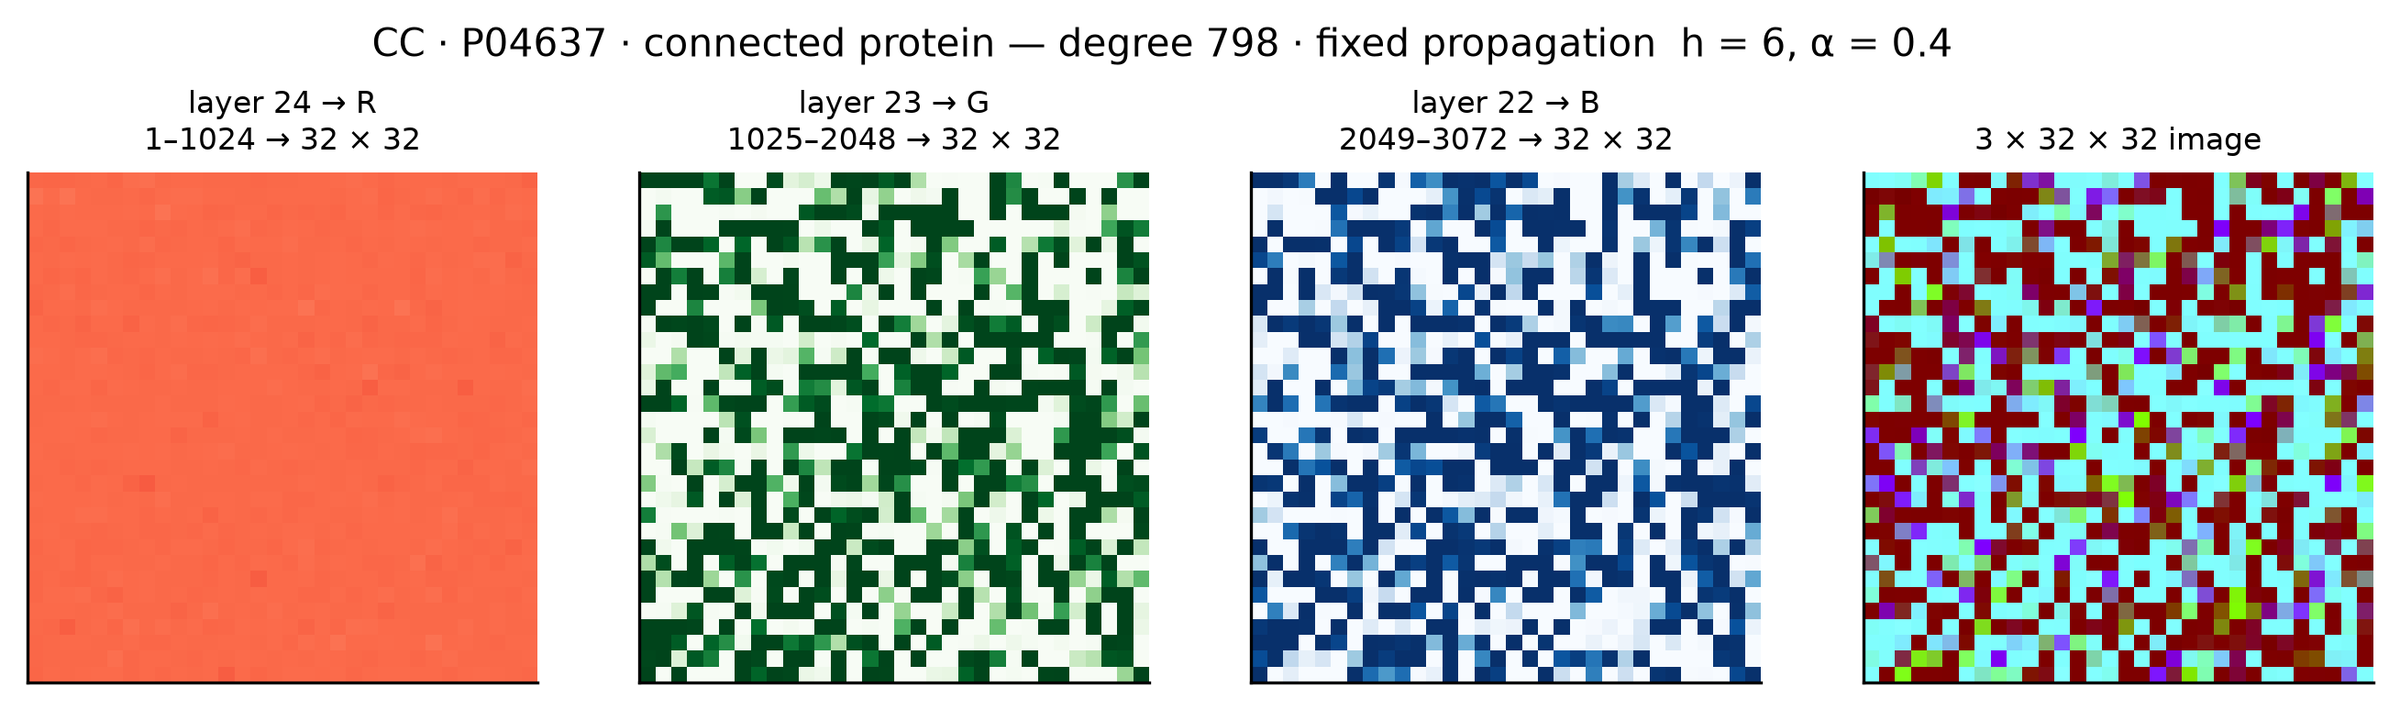
\includegraphics[height=0.3\textheight]{fig_5_9}
    \caption{From a 3072-dimensional vector to a $32\times32\times3$ image.}
  \end{figure}
\end{frame}

\begin{frame}{Training Objective: ProteinLoss}
  \begin{eqbox}[0.7\textwidth]
    $\displaystyle \mathcal{L} = \mathcal{L}_{\mathrm{ZLPR}}\cdot\big(1-wF1^{\mathrm{GO}}\big)\cdot\big(1-wF1^{\mathrm{prot}}\big)$
  \end{eqbox}
  \begin{itemize}\setlength{\itemsep}{0.45em}
    \item ZLPR~\cite{su2022zlpr} separates positive from negative terms at threshold zero
    \item Two soft, IC-weighted $F_1$ factors: one across terms, one across proteins~\cite{liu2024interlabelgo}
    \item Brings training closer to the evaluation criterion
    \item Beats binary cross-entropy by 5.47\,pp on the first-generation mean
  \end{itemize}
\end{frame}

\begin{frame}{Combining the Fixed and Learned Routes}
  \begin{columns}[c]
    \column{0.44\textwidth}
    \begin{figure}
      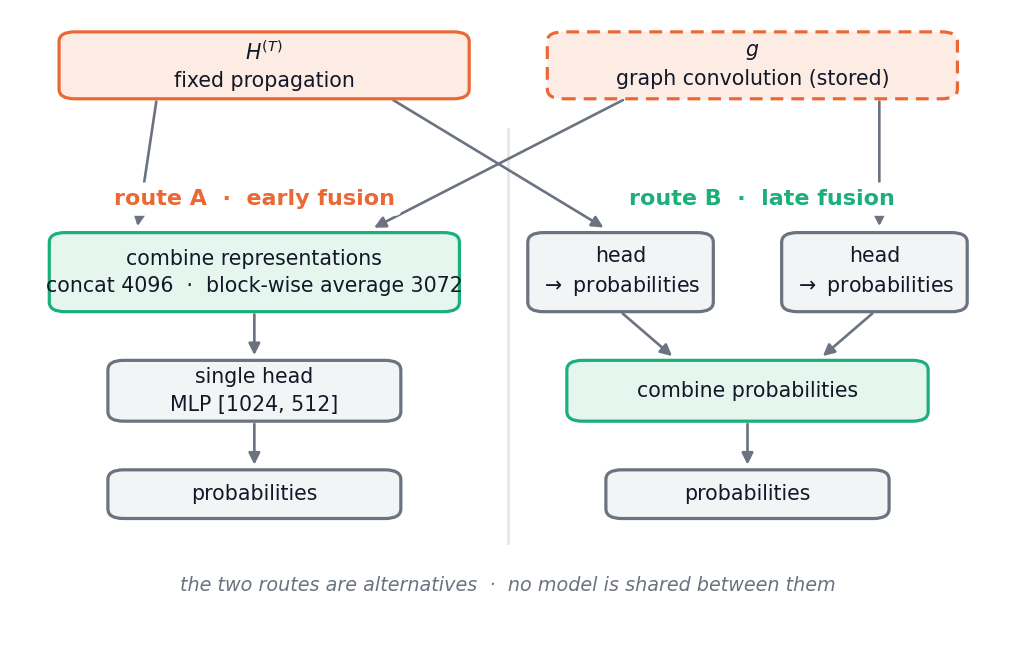
\includegraphics[width=\linewidth]{fig_5_10}
      \caption{Early fusion (left) and late fusion (right).}
    \end{figure}
    \column{0.54\textwidth}
    \begin{itemize}\setlength{\itemsep}{0.35em}\small
      \item \textbf{Early:} join the representations, train one head (concatenation 4096 or block-wise addition 3072)
      \item \textbf{Late:} train each route, combine the probabilities
      \item Eleven late rules: linear $\gamma$, max, min, IC sigmoid, degree sigmoid, master equation and five
        stacking meta-classifiers
      \item Coefficients chosen on validation (71 configurations per ontology)
    \end{itemize}
  \end{columns}
\end{frame}

% =================================================================================== Results
\section{Results and Discussion}

\begin{frame}{Experimental Configuration}
  \begin{itemize}\setlength{\itemsep}{0.3em}
    \item \textbf{Runs:} 170 runs, about 136.3 GPU-hours (147 runs on an RTX A5500)
    \item \textbf{Funnel:} each stage picks its winner on validation and hands it on; the test set is read once
    \item \textbf{Reading:} single seed, so differences below 0.5\,pp are ties
  \end{itemize}
  \vspace{0.5em}
  \begin{table}\scriptsize
    \caption{The order of the decisions and the winner of each stage.}
    \begin{tabular}{@{}lllll@{}}\toprule
      objective & vector architecture & vision backbone & depth $T$ & retention $\alpha$\\
      ProteinLoss & MLP raw & ConvNeXt-Tiny & per ontology & per ontology\\\midrule
      learned encoder & deduplication & early fusion & late fusion & test\\
      GCN & max & add + GCN + vector & linear $\gamma$ & \NX{Late}\\\bottomrule
    \end{tabular}
  \end{table}
\end{frame}

\begin{frame}{Generation 1 Settles Three Choices}
  Mean validation $\wF$:
  \begin{itemize}\setlength{\itemsep}{0.35em}
    \item Naive term-frequency baseline: 43.56
    \item ProteinLoss beats binary cross-entropy: +5.47\,pp on the mean (+8.87 in MF)
    \item MLP on the raw profile wins: 44.51; best 1-D CNN: 41.16
    \item Vision backbones: 36.99 to 37.62
  \end{itemize}
  \vspace{0.5em}
  \begin{block}{Reading}
    Topology alone barely clears a predictor that looks at nothing: +0.95\,pp on the mean.
  \end{block}
\end{frame}

\begin{frame}{Depth and Retention: Vector Head}
  \begin{columns}[c]
    \column{0.49\textwidth}
    \begin{figure}
      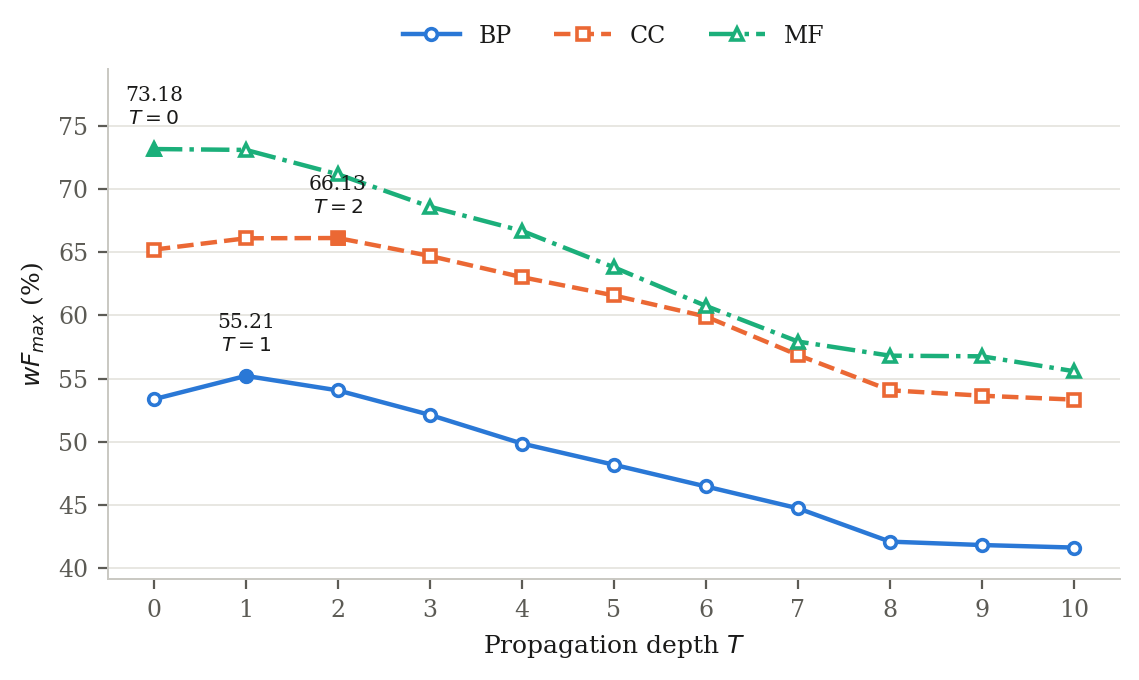
\includegraphics[width=\linewidth]{fig_6_1}
      \caption{Propagation depth $T$.}
    \end{figure}
    \column{0.49\textwidth}
    \begin{figure}
      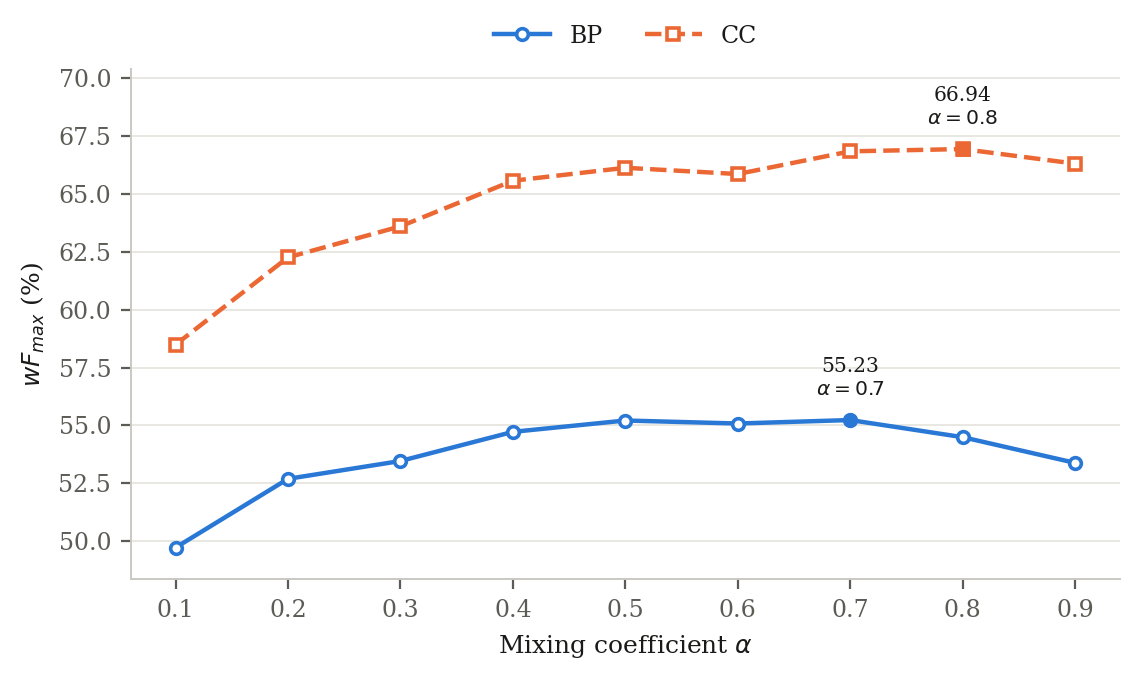
\includegraphics[width=\linewidth]{fig_6_2}
      \caption{Retention coefficient $\alpha$.}
    \end{figure}
  \end{columns}
  \begin{itemize}\small
    \item Peak depth: $T=1$ BP, $T=2$ CC, $T=0$ MF; beyond it, 12.80 to 17.60\,pp lost by $T=10$
    \item Best retention: $\alpha=0.7$ BP, $\alpha=0.8$ CC; the graph corrects the protein's own representation
  \end{itemize}
\end{frame}

\begin{frame}{Depth and Retention: Vision Head}
  \begin{columns}[c]
    \column{0.49\textwidth}
    \begin{figure}
      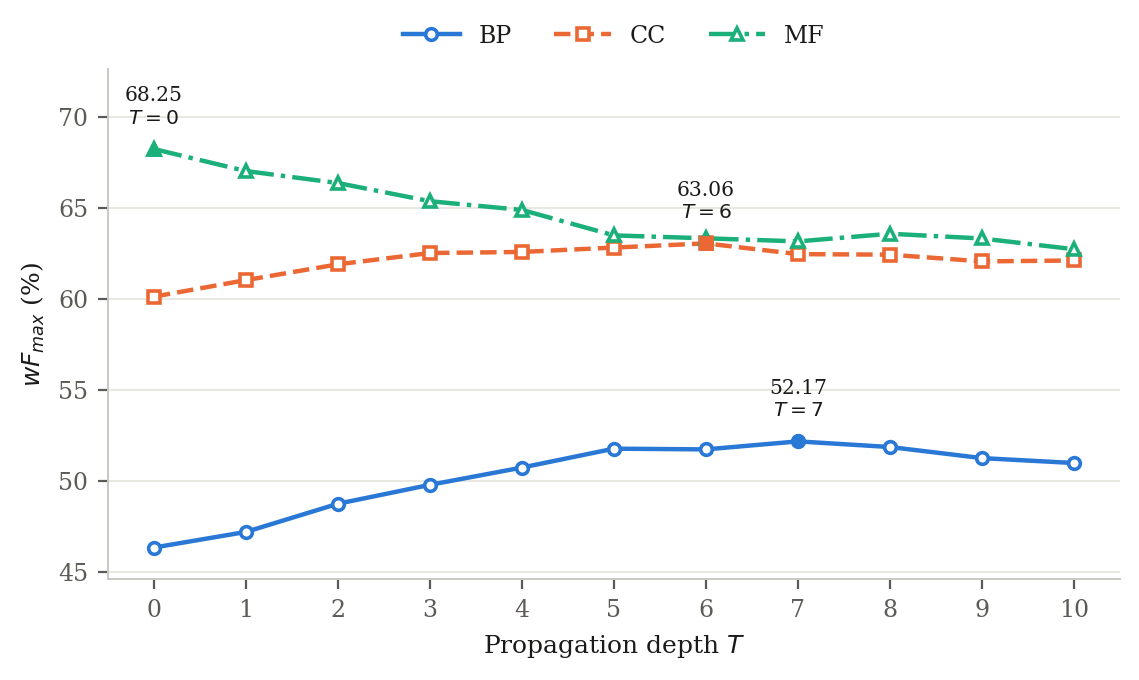
\includegraphics[width=\linewidth]{fig_6_3}
      \caption{Propagation depth $T$.}
    \end{figure}
    \column{0.49\textwidth}
    \begin{figure}
      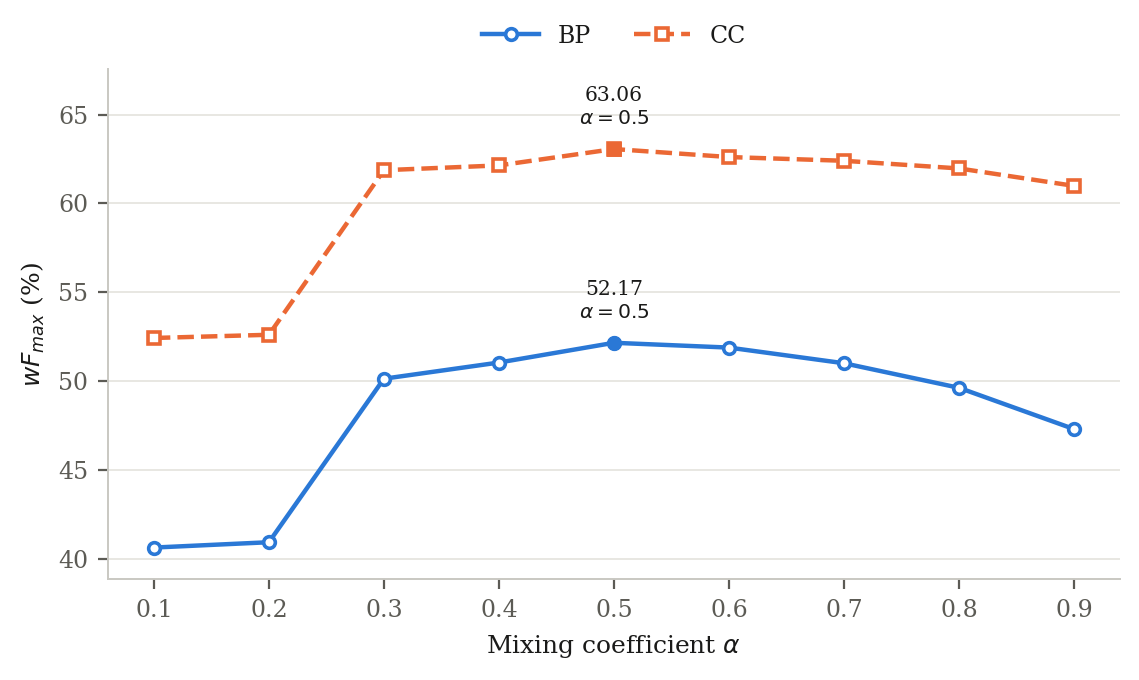
\includegraphics[width=\linewidth]{fig_6_4}
      \caption{Retention coefficient $\alpha$.}
    \end{figure}
  \end{columns}
  \begin{itemize}\small
    \item Peak depth: $T=7$ BP, $T=6$ CC, $T=0$ MF; gains over $T=0$: +5.84 BP, +2.93 CC (vector: +1.85, +0.92)
    \item Its best BP value, 52.17, is still below the vector head's graph-free 53.36
  \end{itemize}
\end{frame}

\begin{frame}{Fixed or Learned Aggregation?}
  \begin{columns}[T]
    \column{0.64\textwidth}
    \begin{table}
      \caption{End-to-end GNN routes, validation $\wF$.}
      \resizebox{\linewidth}{!}{\TabGNN}
    \end{table}
    \begin{itemize}\setlength{\itemsep}{0.3em}\small
      \item GCN beats GAT in all 6 pairs (3.88 to 9.31\,pp), and in 30 of 30 fusion pairs
      \item Deduplication: max never loses beyond noise; GAT gains the most (+3.83 vision)
    \end{itemize}
    \column{0.34\textwidth}
    \vspace{1.2em}
    \only<2>{\callout{\textbf{Fixed} propagation reaches 65.12 mean $\wF$ against 63.32 for the \textbf{GCN}: the GCN
      leads in BP by 0.55 (at the 0.5\,pp floor) and trails in CC by 0.59 and in MF by 5.35.}}
  \end{columns}
\end{frame}

\begin{frame}{Fusion Helps; Combining Predictions Helps More}
  \begin{columns}[T]
    \column{0.52\textwidth}
    \begin{table}
      \caption{Late fusion rules, validation $\wF$.}
      \resizebox{\linewidth}{!}{\TabLate}
    \end{table}
    \column{0.46\textwidth}
    \vspace{0.8em}
    \begin{itemize}\setlength{\itemsep}{0.35em}\small
      \item \textbf{Early}, one configuration (add, GCN, vector): 65.80, +0.68 over fixed alone
      \item \textbf{Late}, linear $\gamma$ (0.50 BP, 0.55 CC and MF): 67.06, best in every ontology
      \item Gains over the better component: +2.18 BP, +1.85 CC, +1.26 MF
    \end{itemize}
    \vspace{0.5em}
    \only<2>{\callout{In the stacking models, the two route probabilities carry almost all the weight.}}
  \end{columns}
\end{frame}

\begin{frame}{Vector Head Wins 12 of 12}
  \begin{columns}[T]
    \column{0.64\textwidth}
    \begin{table}
      \caption{Vector and vision heads at each stage, validation $\wF$.}
      \resizebox{\linewidth}{!}{\TabVV}
    \end{table}
    \column{0.34\textwidth}
    \vspace{1.2em}
    \begin{itemize}\small
      \item Margin on the mean: +6.62, +3.96, +2.69 and +3.35\,pp across the four stages, with no trend toward zero
    \end{itemize}
    \vspace{0.5em}
    \only<2>{\callout{Neither image has the locality a convolution assumes: the vector head wins every stage and
      ontology.}}
  \end{columns}
\end{frame}

\begin{frame}{Where the Gains Come From}
  \begin{center}
  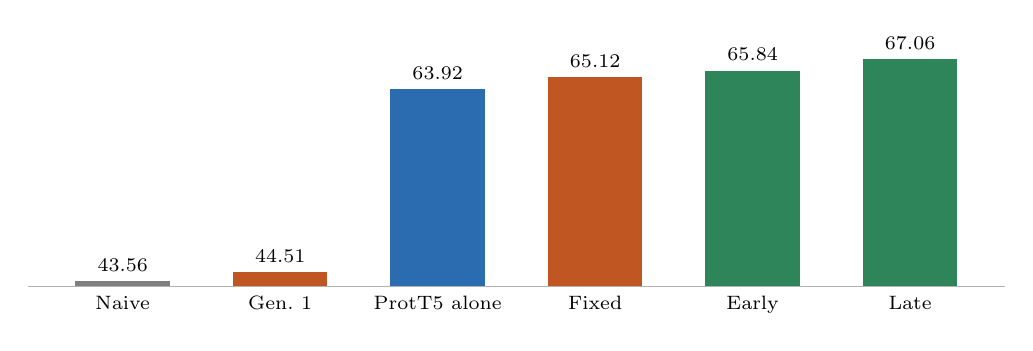
\begin{tikzpicture}[x=2.0cm, y=0.12cm, font=\small]
    \draw[gray!60] (0.4,43) -- (6.6,43);
    \foreach \i/\v/\c/\l in \GainBars {
      \fill[\c] (\i-0.3,43) rectangle (\i+0.3,\v);
      \node[above, font=\scriptsize] at (\i,\v) {\v};
      \node[below, font=\scriptsize] at (\i,43) {\l};
    }
  \end{tikzpicture}
  \end{center}
  {\scriptsize Mean validation $\wF$; axis starts at 43. Blue: sequence; orange: network; green: fusion.
  Early: best configuration per ontology.}
  \begin{block}{Reading}
    Most of the jump comes from the language model; the graph adds the rest.
  \end{block}
\end{frame}

\begin{frame}{Test Set: Comparison with the Literature (BP)}
  \begin{columns}[T]
    \column{0.66\textwidth}
    \begin{table}\scriptsize
      \caption{Test set, Biological Process.}
      \resizebox{\linewidth}{!}{\TabTestBP}
    \end{table}
    \column{0.32\textwidth}
    \vspace{1.5em}
    \begin{overprint}
      \onslide<2>\callout{\NX{Late} leads the strongest baseline, DeepGraphGO, by 9.77\,pp of $\wF$; $\Smin$ agrees:
        17.12 against 20.11 bits.}
      \onslide<3>\callout{The \textbf{ProtT5 baseline} alone already beats every literature method on $\wF$.}
      \onslide<4>\callout{Fixed propagation adds 1.87\,pp over the ProtT5 baseline: the graph corrects the sequence
        representation.}
    \end{overprint}
  \end{columns}
\end{frame}

\begin{frame}{Test Set: Comparison with the Literature (CC)}
  \begin{columns}[T]
    \column{0.66\textwidth}
    \begin{table}\scriptsize
      \caption{Test set, Cellular Component.}
      \resizebox{\linewidth}{!}{\TabTestCC}
    \end{table}
    \column{0.32\textwidth}
    \vspace{1.5em}
    \begin{overprint}
      \onslide<2>\callout{\NX{Late} leads the strongest baseline, DeepGraphGO, by 8.67\,pp of $\wF$; $\Smin$ agrees:
        8.22 against 9.67 bits.}
      \onslide<3>\callout{The topology-only \textbf{First Generation} trails the ProtT5 baseline by 16.39\,pp: most of
        the gain comes from the language model.}
      \onslide<4>\callout{Fixed propagation adds 2.15\,pp over the ProtT5 baseline: the graph complements the
        sequence.}
    \end{overprint}
  \end{columns}
\end{frame}

\begin{frame}{Test Set: Comparison with the Literature (MF)}
  \begin{columns}[T]
    \column{0.66\textwidth}
    \begin{table}\scriptsize
      \caption{Test set, Molecular Function.}
      \resizebox{\linewidth}{!}{\TabTestMF}
    \end{table}
    \column{0.32\textwidth}
    \vspace{1.5em}
    \begin{overprint}
      \onslide<2>\callout{\NX{Late} leads the strongest baseline, DeepGraphGO, by 4.93\,pp of $\wF$; $\Smin$ agrees:
        5.14 against 5.67 bits.}
      \onslide<3>\callout{ProtT5 baseline and \NX{Fixed} are the same run: the best depth in MF is $T=0$. Only the
        fusion routes improve on its $\wF$, modestly.}
      \onslide<4>\callout{Across the three ontologies, \NX{Late} is best in every column except AuPRC in MF, where
        \NX{Early} leads by 5.35\,pp.}
    \end{overprint}
  \end{columns}
\end{frame}

\begin{frame}{Every Protein Gets a Prediction}
  \begin{table}\small
    \caption{Prediction coverage of the test split by method family.}
    \TabCov
  \end{table}
  \begin{itemize}\setlength{\itemsep}{0.35em}
    \item DeepGraphGO and SEGT-GO reach unseen proteins through homology search
    \item Mashup, MELISSA and deepNF score only network members; missing proteins count as misses
    \item Part of the distance to network-only methods is reach, not ranking quality
  \end{itemize}
\end{frame}

\begin{frame}{Computational Cost}
  \begin{columns}[c]
    \column{0.5\textwidth}
    \begin{figure}
      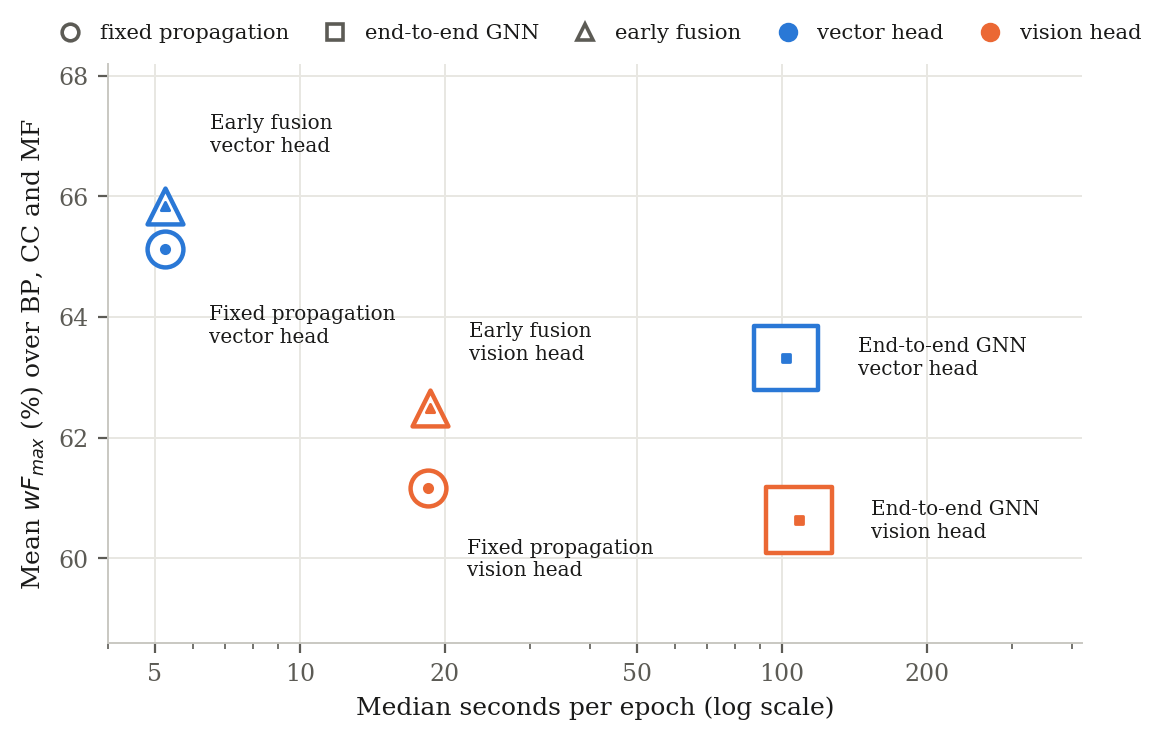
\includegraphics[width=\linewidth]{fig_6_5}
      \caption{Mean $\wF$ against median seconds per epoch (log scale).}
    \end{figure}
    \column{0.48\textwidth}
    \begin{itemize}\setlength{\itemsep}{0.35em}\small
      \item Fixed + vector: 5.24\,s/epoch, 6.4\,GiB peak
      \item GCN alone: 68.76\,s/epoch, 14.1\,GiB; GAT: 161.41\,s, 20.7\,GiB
      \item \alert{Matches or beats the GCN at about 1/13 of the time and under half the memory}
      \item Early fusion costs the same as fixed propagation once $g$ is stored
    \end{itemize}
  \end{columns}
\end{frame}

\begin{frame}{The Graph Helps Where There Is Graph}
  \begin{columns}[c]
    \column{0.54\textwidth}
    \begin{figure}
      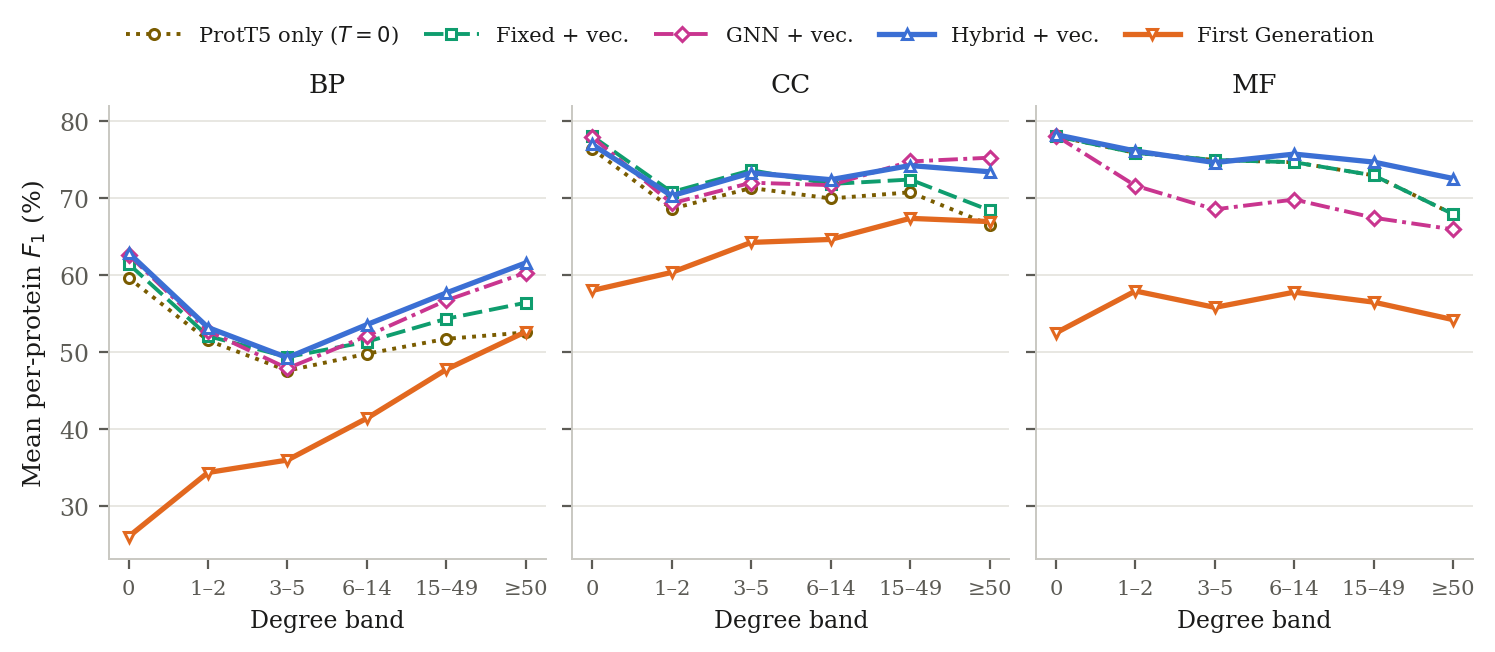
\includegraphics[width=\linewidth]{fig_6_6}
      \caption{Per-protein $F_1$ by degree band, test set.}
    \end{figure}
    \column{0.44\textwidth}
    \begin{table}
      \caption{Gain over the $T=0$ control (per-protein $F_1$, test, pp); f fixed, g GNN, h early fusion.}
      \resizebox{\linewidth}{!}{\TabGain}
    \end{table}
  \end{columns}
  \begin{itemize}\small
    \item Every ProtT5 route scores worse on connected than on isolated proteins; the graph-free control shows it too
    \item The graph's gain grows with degree: up to +9.05 BP, +8.71 CC, +4.64 MF at degree $\ge 50$
  \end{itemize}
\end{frame}

% =================================================================================== Conclusions
\section{Conclusions and Contributions}

\begin{frame}{General Conclusions}
  \begin{itemize}\setlength{\itemsep}{0.45em}\small
    \item \textbf{Language model first:} most of the gain comes from ProtT5 (44.51 for the network alone, 63.92 for
      ProtT5 alone, mean validation $\wF$); the graph adds the rest.
    \item \textbf{Fixed matches learned:} fixed propagation (65.12) matches or beats the GCN (63.32) at about 1/13 of
      the time per epoch.
    \item \textbf{Fusion pays:} late fusion reaches 67.06, the best in every ontology (validation).
    \item \textbf{Vector head:} wins 12 of 12 comparisons; the images impose a locality the data lacks.
    \item \textbf{The graph helps where there is graph:} the gain grows with degree, up to +9.05\,pp in BP.
  \end{itemize}
\end{frame}

\begin{frame}{Answers to the Research Questions (1/2)}
  \begin{itemize}\setlength{\itemsep}{0.55em}\small
    \item \textbf{(RQ1) Which representation of the STRING network works best?}\\
      The unreduced interaction profile with an MLP; imposed locality hurts.
    \item \textbf{(RQ2) How much does propagating ProtT5 embeddings over STRING add?}\\
      A large gain, mostly from ProtT5; propagation adds +1.87 BP, +2.15 CC and nothing in MF (test).
    \item \textbf{(RQ3) Fixed or learned aggregation, vector or image heads?}\\
      Late 67.06 $>$ Early 65.84 $>$ Fixed 65.12 $>$ GNN 63.32 (validation); the vector head throughout.
    \item \textbf{(RQ4) Do early and late fusion improve on their components?}\\
      Both help; late fusion more: +1.26 to +2.18\,pp over the better component (validation).
  \end{itemize}
\end{frame}

\begin{frame}{Answers to the Research Questions (2/2)}
  \begin{itemize}\setlength{\itemsep}{0.55em}\small
    \item \textbf{(RQ5) How deep should the propagation go, and how much should a protein retain?}\\
      One or two hops with $\alpha$ between 0.7 and 0.8; MF prefers no propagation.
    \item \textbf{(RQ6) How does the approach compare with the literature, on the same splits?}\\
      Best in every column but one; $\wF$ margins of +9.77, +8.67 and +4.93\,pp (test).
    \item \textbf{(RQ7) Does it work on one global, aggregated-evidence network?}\\
      Yes, on one global aggregated network; graphs partitioned by organism or evidence were not tested.
  \end{itemize}
\end{frame}

\begin{frame}{Limitations of the Study}
  \begin{itemize}\setlength{\itemsep}{0.45em}
    \item Single seed: the 0.5\,pp floor is a reading convention, not a confidence interval
    \item Random protein-level split: transductive interpolation, possible homology leakage
    \item STRING scores may encode annotation knowledge (circularity)
    \item Fixed against learned is not a single-factor ablation ($\alpha^{T}$ scaling, normalization)
    \item Baselines adapted to one aggregated network and a reduced label space
  \end{itemize}
\end{frame}

\begin{frame}{Future Work}
  \begin{itemize}\setlength{\itemsep}{0.45em}
    \item Separate the graph by organism, or train one model per organism
    \item Keep the STRING evidence channels apart (typed or parallel edges)
    \item Heterogeneous graphs of proteins, terms and evidence; compare with ProtHGT~\cite{ulusoy2025prothgt}
    \item Sampled aggregation (GraphSAGE~\cite{hamilton2017graphsage}) for a cheaper learned route
    \item Richer node features: structure, domains, expression; most promising for MF
  \end{itemize}
\end{frame}

\begin{frame}{Contributions and Publications}
  \textbf{Scientific contributions:}
  \begin{itemize}\setlength{\itemsep}{0.15em}\small
    \item \textbf{Method:} NEXUS-GO, a non-parametric multi-hop propagation of ProtT5 embeddings over STRING
    \item \textbf{Controlled comparisons:} fixed against learned (GCN, GAT) aggregation; vector against image heads
    \item \textbf{Fusion:} early and late fusion of the two routes; linear late fusion gives the best $\wF$ of the work
    \item \textbf{Benchmark:} five network-based methods retrained on the same splits and transductive setting
  \end{itemize}
  \vspace{0.3em}
  \textbf{Academic output:}
  \begin{itemize}\setlength{\itemsep}{0.15em}\small
    \item Paper published at \textbf{VISAPP 2026} (Marbella, Spain)~\cite{mauhnoom2026graphs}
    \item Extended version accepted in \textbf{Communications in Computer and Information Science}, expected in
      December 2026~\cite{mauhnoom2026beyond}
    \item Code: \texttt{github.com/ymauhn/nexus-go}
  \end{itemize}
\end{frame}

\begin{frame}[allowframebreaks]{References}
  \scriptsize
  \bibliographystyle{abbrv}
  \bibliography{references}
\end{frame}

\begin{frame}{Acknowledgements}
  \begin{itemize}\setlength{\itemsep}{0.35em}\small
    \item My advisor, Prof.\ Dr.\ Zanoni Dias, and my co-advisors, Prof.\ Dr.\ Hélio Pedrini and Dr.\ Gabriel
      Bianchin de Oliveira, for their guidance
    \item My family, especially my parents, and my friends and colleagues, for their support
    \item CAPES and BTG Pactual, for the financial support
    \item The Institute of Computing of Unicamp, for the computational resources
  \end{itemize}
  \vfill
  \begin{columns}[c]
    \column{0.5\textwidth}\centering
    
\includegraphics[height=2.0cm]{logo-unicamp}\\[0.3em]
    {\small University of Campinas (Unicamp)}
    \column{0.5\textwidth}\centering
    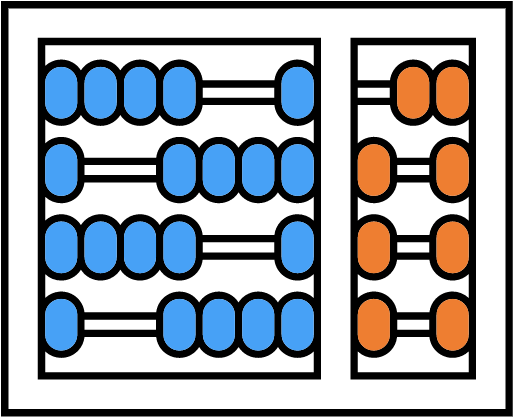
\includegraphics[height=1.6cm]{logo-ic}\\[0.5em]
    {\small Institute of Computing (IC)}
  \end{columns}
  \vfill
\end{frame}

\begin{frame}
  \titlepage
\end{frame}

% =================================================================================== Backup
\appendix
\section*{Backup}

\begin{frame}{Backup: Computational Cost by Family}
  \begin{table}\scriptsize
    \caption{RTX A5500, 147 runs; lowest value in bold for s/epoch, h/run and VRAM.}
    \TabCost
  \end{table}
\end{frame}

\begin{frame}{Backup: Deduplication of STRING Records}
  \begin{itemize}\setlength{\itemsep}{0.45em}
    \item Symmetric weights, no self-loops, sparse COO storage ($\le$ 1.13\,M stored entries; dense would take
      25 to 35\,GB)
    \item \textbf{max} keeps the score; \textbf{sum} multiplies it by the record count
  \end{itemize}
  \begin{block}{Example}
    Neighbour A (score 0.80, 5 records) and B (0.95, 1 record). With sum, A weighs 4.00 against 0.95 and dominates;
    with max, B (0.95) ranks above A (0.80). Normalization does not undo the reordering.
  \end{block}
\end{frame}

\end{document}
